\documentclass[lettersize,journal]{IEEEtran}
\usepackage{amsmath,amsfonts}
\usepackage{algorithmic, algorithm}
% \usepackage[ruled,vlined,linesnumbered]{algorithm2e}
\usepackage{array}
\usepackage[caption=false,font=normalsize,labelfont=sf,textfont=sf]{subfig}
\usepackage{textcomp}
\usepackage{stfloats}
\usepackage{url}
\usepackage{verbatim}
\usepackage{graphicx}
\usepackage{cite}
\usepackage{tabularx}
\usepackage{multirow, makecell}
\graphicspath{{figures/}}
\hyphenation{op-tical net-works semi-conduc-tor IEEE-Xplore}


\begin{document}

\title{Deep Reinforcement Learning-based Joint Caching and Offloading Scheme in Vehicular Edge Computing Systems for Tasks With Heterogeneous Service Requirements}







% \author{ ~\IEEEmembership{Staff}
%         % <-this % stops a space
% \thanks{This paper was produced by the IEEE Publication Technology Group. They are in Piscataway, NJ.}% <-this % stops a space
% \thanks{Manuscript received April 19, 2021; revised August 16, 2021.}}

\author{ ~\IEEEmembership{IEEE}}

% The paper headers
% \markboth{Journal of \LaTeX\ Class Files,~Vol.~14, No.~8, August~2021}%
% {Shell \MakeLowercase{\textit{et al.}}: A Sample Article Using IEEEtran.cls for IEEE Journals}

%\IEEEpubid{0000--0000/00\$00.00~\copyright~2021 IEEE}
% Remember, if you use this you must call \IEEEpubidadjcol in the second
% column for its text to clear the IEEEpubid mark.

\maketitle






\begin{abstract}
In recent years, vehicular edge computing (VEC) has emerged as a promising paradigm.
% Existing studies mainly focus on offloading scenarios where each task requests only a single type of service and often ignore fine-grained task decomposition.
% Therefore, they are incapable of handling heterogeneous service requirements, leading to inefficient utilization of edge's caching resources.
% Existing studies mainly focus on offloading tasks requesting a single service without considering fine-grained task decomposition, making them incapable of handling heterogeneous service requirements and leading to inefficient utilization of edge caching resources.
% Existing studies mainly focus on offloading scenarios where each task requests only a single type of service, thereby failing to support heterogeneous service requirements from the same task.
In previous studies on offloading in VEC, a task is always supposed to only request one type of service, limiting the universality of research.
To address these limitations, we propose a deep reinforcement learning (DRL)-based joint  service caching and task offloading scheme, named DRLSCCO.
The advantages of the proposed scheme are as follows: 1) it allows each task to request multiple types of services simultaneously, 2) it enables fine-grained task decomposition based on service types and distributed offloading of subtasks, and 3) it supports both cloud collaboration and edge collaboration.
To comprehensively evaluate the performance of the proposed DRLSCCO scheme, we conduct extensive comparative  experiments against four benchmark schemes. 
First, we investigate the convergence behavior of different schemes under dynamic task size and vehicle density.
Second, by varying task size and vehicle density, respectively, we reveal the variation  pattern of task delay underlying the governing of these factors.
Third, with vehicle density and task size held constant, we explore  the impact of edge server CPU frequency on energy consumption of mobile network operators (MNOs).
Results demonstrate that DRLSCCO outperforms the four benchmark schemes in reducing task delay  under various parameter configurations, and achieves the slowest increase of energy consumption as edge server CPU frequency increases.
\end{abstract}
\begin{IEEEkeywords}
Service caching, task offloading, vehicular network, deep reinforcement learning.
\end{IEEEkeywords}


\section{Introduction}
%写VEC出现,VEC内容缓存和服务缓存是什么
\IEEEPARstart{W}{ith}
the rapid development of autonomous vehicles (AVs) and the internet of things (IoT), the internet of vehicles (IoV) has emerged as an integrated network connecting vehicles, small cloud servers deployed at roadside units (RSUs), and centralized cloud systems. The IoV enable various communication modes and foster the deployment of computation-intensive and latency-sensitive vehicular applications. \cite{Xing-1, TalebkhahSali-2}.
%**这些应用计算密集, 延迟敏感, 车辆能力有限, 远程云延迟高, 回程链路负载大**
Due to the limited computing and caching resources of vehicles, as well as the high latency and backhaul overhead associated with cloud computing, supporting such applications remains challenging \cite{WaheedShah-3}.

% **幸运的是有VEC** 
Fortunately, researchers have integrated edge computing into the IoV, leading to the development  of vehicular edge computing (VEC) \cite{LiuChen-5, WuWang-6, M.S.-7}. 
%**简述VEC处理任务的好处**
This architecture enables vehicles migrate applications to the RSUs equipped with edge server  or request popular content from these RSUs, reducing task execution and content request delays.
% 
%\IEEEpubidadjcol
Despite the numerous advantages of VEC, edge servers still suffer from significantly limited computing and caching resources compared to centralized cloud servers \cite{Reiss-MirzaeiGhobaei-Arani-13, KhanMustafa-14}. 
To overcome this limitation, a cloud-edge collaborative vehicular edge computing (VEC) framework has been applied \cite{YanLi-17, RenChen-19}.
Under this framework, vehicular tasks can be executed locally, offloaded to nearby edge servers or further forwarded to centralized cloud servers.
Most existing works based on this framework focus primarily on content caching strategies, task offloading schemes or their integration. However, they  overlook the crucial role of service caching in enabling efficient task offloading within VEC, especially given the limited caching resources of edge servers \cite{MaoYou-12}.

Service caching  storing specific service programs required by vehicular applications to minimize the delay associated with service requests and application initialization, thereby improving the quality of experience (QoE).
In fact, task execution fundamentally depends on service caching: a task can only be processed by vehicles or edge servers that have already cached the corresponding service program. This dependency creates a strong coupling between service caching and task offloading decisions.
Moreover, vehicular tasks exhibit significant variability in service dependencies, making preconfigured caching and offloading decisions infeasible. 
These technical challenges are further amplified by the rapid proliferation of new energy vehicles and their associated smart applications. These applications often integrate multiple functions—each corresponding to a distinct service program—and thus exacerbate the caching burden on edge servers \cite{ShiCao-8}.
Therefore, there is an urgent need for a service caching and task offloading scheme to address these challenges.
However, many existing studies still rely on greedy heuristics or offline optimizations, which struggle to handle the dynamic characteristics of vehicular networks. 
Although some researchers have employed reinforcement learning to assist decision-making, the assumption that each task depends on a single type of service fails to capture the requirements of multi-function applications.

%**针对上述问题, 本文将怎样怎样.....**
To address the aforementioned issues, we focus on a cloud-edge collaborative VEC framework
and propose a deep reinforcement learning (DRL)-based joint service caching and task offloading scheme, named DRLSCCO. 
Specifically, a service-based task decomposition mechanism is introduced, where each task is decomposed into multiple subtasks according to different service programs, allowing flexible offloading based on distributed service caches. 
The joint decision-making process is formulated as a markov decision process (MDP), where the system state captures the dynamic network conditions, including vehicle density, service caching states, and heterogeneous task demands. The action space simultaneously determines the service caching and task offloading decisions across vehicles and edge nodes.
To handle the high-dimensional, continuous decision space, we adopt the deep deterministic policy gradient (DDPG) algorithm to learn an adaptive policy that minimizes the cumulative average task execution delay.
The main contributions of this paper are summarized as follows: 
\begin{enumerate}
	\item 
	We propose a novel cloud-edge collaborative VEC framework that incorporates a service-based task decomposition mechanism. It allows each task to request multiple types of services simultaneously and  fine-grained task decomposition based on service types.
	To minimize the cumulative average task execution latency, the joint service caching and fine-grained task offloading optimization problem is formulated as a mixed-integer nonlinear programming (MINLP) problem, which considers heterogeneous service requirements of tasks, caching constraints at vehicles and edge nodes.

	\item 
	Given the NP-hardness of the formulated problem, we design the DRLSCCO scheme, which is capable of jointly optimizing caching and offloading decisions under continuous and high-dimensional system states. Unlike prior works that decouple caching and offloading, our scheme jointly learns service caching and task offloading decisions in a continuous, high-dimensional action space, capturing the interdependencies between the two.
	
	\item We conduct extensive experiments under varying conditions, including task size, vehicle density and edge server CPU frequency, to validate the adaptability and effectiveness of our proposed DRLSCCO scheme. The results show that DRLSCCO outperforms the four benchmark schemes in reducing task delay across diverse scenarios and
	exhibits minimum growth rate of energy consumption as edge server CPU frequency increases.
\end{enumerate}


The rest of this paper is organized as follows. Section II reviews the related work. Section III introduces the system model and formulates the MINLP problem. Section IV presents the proposed DRLSCCO scheme in detail. Section V provides simulation results and performance analysis. Finally, Section VI concludes the paper and outlines directions for future research.

\section{Related Work}
\subsection{Studies on MEC}
In recent years, computation offloading  has emerged as a research hotspot in mobile edge computing (MEC) \cite{Raeisi-VarzanehDakkak-23}.
% 
To minimize time cost while ensuring low computational delay and high reliability, Lin et al. \cite{LinHuang-24} proposed a Lyapunov-based resource allocation scheme in unmanned aerial vehicles (UAVs)-assisted heterogeneous edge computing system.
% 
Zhang et al. \cite{L-29} utilized  Lagrangian relaxation (LR) in the bidirectional task offloading model, formulating the problem of minimizing the average bandwidth as an auxiliary problem to obtain a locally optimal solution.
% 
Nevertheless, traditional optimization methods often struggle to adapt to the highly dynamic MEC environments. To overcome this, reinforcement learning (RL) techniques have been widely adopted to derive adaptive strategies through online interactions.
% 
Zhang et al. \cite{ZhangXia-25} developed  a DRL-based offloading strategy for latency-sensitive home devices to reduce system costs and enhance user experience.
% 
Zeng et al. \cite{ZengWang-26} proposed a three-layer cloud-edge-end collaboration (CEEC) architecture, jointly optimizing offloading strategies, computing resources, and network channels under a newly defined QoE metric.
% 
To cope with the resource-sharing nature of specialized tasks, Xie et al. \cite{XieFang-27} modeled granularity decisions as a multi-armed bandit problem and applied RL to effectively reduce edge server costs.
% 
Tang et al. \cite{TangWong-28} further proposed a fully distributed DRL-based scheme where each device independently determines its offloading strategy, significantly reducing packet loss and execution delay.



% ---------------------------------------------------------
In parallel with the advances in computation offloading, substantial research has been devoted to edge caching for improving content or service delivery efficiency in MEC systems.
% 
Bounaira et al. \cite{BounairaAlioua-30} addressed the privacy security concerns arising from the lack of trust  between content providers and edge servers in a blockchain-based trust management system.
% 
Beyond privacy security, fairness in cache allocation has also attracted attention. Zhou et al. \cite{ZhouChen-31} investigated the fair edge data caching (FEDC) problem arising from limited storage and vendor competition, while Tang et al. \cite{Tang} introduced a genetic algorithm-based two-level caching and offloading method to ensure equitable resource distribution.
% 
The dynamic nature of content popularity presents additional issues. Mao et al. \cite{MaoHe-32} designed a collaborative meta-learning framework (CMCES) that leverages selective neighbor sampling to improve adaptability, achieving a 10.12\% increase in cache hit rate.
%
Then Zhao et al. \cite{ZhaoNakhai-33} proposed a two-phase proactive caching approach to address uncertain task requirements resulting from the constantly changing content popularity,  improving request prediction accuracy.
%

In summary, MEC has been widely investigated to reduce task delay or improve content delivery efficiency. However, most existing MEC studies focus on relatively static or low-mobility scenarios. In contrast, VEC feature highly dynamic topologies, rapidly changing wireless channels, and stringent delay requirements. These characteristics make direct application of traditional MEC approaches suboptimal in VEC scenarios, thereby motivating dedicated research on VEC-oriented caching and offloading strategies.


\subsection{Studies on VEC}
% VEC

Recent studies have begun to investigate VEC-specific solutions.
In the following, we review representative works on VEC caching and computation offloading.
%
To address energy concerns from the perspective of mobile network operators (MNOs), Kong et al. \cite{KongDuan-10} adopted the DDPG algorithm for joint computing and caching resource allocation.
%
Similarly, Chen et al. \cite{ChenBhargava-9} proposed a hybrid optimization framework combining deep Q-network (DQN) for task offloading with a greedy strategy for resource management, The framwork effectively reduced  system energy consumption under delay constraints.
% 
Beyond centralized solutions, distributed learning techniques have gained progress in facilitating collaborative caching and offloading.
% 
For instance, Wu et al. \cite{WuFan-15} proposed a social-aware decentralized cooperative caching (SADC) algorithm that leverages vehicle social networks to estimate contact rates to reduce the average content access delay.
% 
To enhance caching performance, Wu et al. \cite{WuWang-16} designed a multi-agent federated DRL-based collaborative caching strategy (MFDRL-CCS). This approach employs recurrent neural networks (RNN) to select optimal caching vehicles (CVs) and uses a multi-head attention popularity prediction (MHAPP) model to forecast content demand.
% 

The abovementioned studies on VEC mainly focus on terrestrial vehicular networks, while researchers has extended the VEC architecture into more heterogeneous and hierarchical environments.
%
Yu et al. \cite{YuGong-11} conducted the first survey on edge computing in space-air-ground-integrated networks (SAGINs). They applied an offline deep imitation learning (DIL) algorithm to enable real-time caching and offloading decisions, and also discussed potential integration directions for edge computing in SAGINs.
% 
Similarly, Yu et al.\cite{YuWu-35} addressed high-traffic density by integrating UAVs into cellular networks for cooperative caching. The authors used a temporal-evolving bipartite graph neural network (TBGN) to predict mobility patterns and optimize UAV trajectories.

In addition to content caching, service caching has emerged as a critical component in VEC due to its requirement for both storage and computation resources.
Xue et al. \cite{XueLiu-18} proposed a DRL-based joint service caching and task offloading scheme that emphasizes the inherent coupling between service caching and computation task decisions.
% 
Extending this foundation, Liu et al. \cite{L.Z.-4} investigated a model with linearly related requests where the output of one task serves as the input for the next. They analyzed the impact of various factors on task execution latency and system energy consumption.
% 
Cheng et al. \cite{ChengZhai-36} proposed a CO-MATCH algorithm, which integrates dynamic programming-based service caching (DPSC) with a many-to-one matching game (MOMG) for computation offloading. This algorithm jointly considers service caching preferences and social similarity to minimize the overall task processing cost.
% 
Service caching preferences are also considered by  Ling et al. \cite{LingZhang-21}  with particular emphasis on this aspect. They developed a transportation-aware, data-driven cache replacement mechanism that dynamically adapts to real-time changes in vehicle mobility and service preferences.
% 

Although VEC has been extensively studied, literature focusing on the joint optimization of service caching and task offloading remains limited. 
Furthermore, most existing works assume that edge nodes possess sufficient  caching resources, with only a few works incorporating explicit upper bounds on caching capacities \cite{XueLiu-18,L.Z.-4}.
Among these studies that incorporate resource constraints, offloading decisions only depend on a single type of cached service.
To fill this gap, this paper jointly optimizes service caching and task offloading with constrained caching and computing resources of both vehicles and edge nodes. 
Specifically, we consider a task model in which each task may require multiple types of services. To capture the highly dynamic nature of vehicular environments, we simulate scenarios by varying key parameters such as task sizes and edge server computing capacities. Our objective is to minimize the average task delay while maintaining a low growth rate of MNO's energy consumption.

\section{System Model}
In this section, we first provide an overview of our system.  
Then, we elaborate on the system from three perspectives: the communication model, the service dependency generation model, the joint service caching and computation offloading model, and the task processing delay and energy consumption model.  
Next, we analyze the extremum values of delay and energy consumption to gain insights into the task execution delay and MNOs' energy consumption under different caching scenarios.  
Finally, we formulate the optimization problem. For better readability, the main notations used in this paper are summarized in Table~\ref{tab: notations}.
\begin{table}
	\caption{Main Notations}
	\label{tab: notations}
	\begin{center}
	% \renewcommand\arraystretch{1.2}
	\begin{tabularx}{\linewidth}{p{1.8cm} X}
	\hline
	\textbf{Notation} & \textbf{Meaning}  	\\ \hline
	$ \mathcal{L} $ 			& The set of vehicles   								\\
	$ L $ 						& The total number of vehicles   						\\	
	$ \mathcal{N} $ 			& The set of RSUs  										\\	
	$ N $ 						& The total number of RSUs  						\\	
	$ \mathcal{C}_{n} $			& The set of cooperative edge nodes for edge node $ n $  \\	
	$ \mathcal{T} $				& The set of time slots		   							 \\
	$ T $						& The total number of time slots for each episode					 \\		
	$ \mathcal{K} $				& The set of service program types	    			\\	
	$ \mathcal{J}_t $			& The set of tasks  at time slot $ t $	    			\\
	$ d_j $						& The input data size of task  $ j $	   		 \\	
	$ d_{j,k} $				& The input data size of type-$ k $ subtask for task $ j $ \\
	$ f_{j,k} $				& The dependency variable of task $j $ with  type-$ k $  service
	\\	
	$ b_{l,n} $				& The bandwidth allocated to vehicle $ l $ by edge node $ n $ 																					\\	
	% $ \beta $					& The data size of each service program			\\	
	% $ \delta^{R}_{n,k} $			& The caching sate (decision) of edge node $ n $ for $ k $-th service \\
	% $ S^{V} $						&	The storage resource of vehicle (edge node) 	\\
	$ \delta^{V}_{l,k}  $			&	The cache hit state of vehicle $ l$ for type $ k $ service		\\	
	$ \delta^{R}_{n,k} $				& The cache hit state of edge node $ n $ for type $ k $ service 		\\
	$ f^{V}$					&	The max CPU frequency of each vehicle 	\\	
	$ f^{R} $					&  The max CPU frequency of each edge node\\
	% $ \lambda $							&	The CPU cycles required to compute $ 1 $ bit of task data 	\\	
	% $ \kappa$							&	The energy efficiency parameter		\\
	$ \omega^{V}_{l,j,k}$			&	The offloading proportion of vehicle-to-edge	\\	
	$ \omega^{R}_{n,j,k}$			&	The offloading proportion of edge-to-edge\\	
	\hline
	\end{tabularx}
	\end{center}
\end{table}

\subsection{System Overview}
It is assumed that each edge node obtains complete information about the vehicles within its coverage area, and that the coverage areas of different edge nodes are non-overlapping, collectively covering the entire road network.
As illustrated in Fig. \ref{fig: system model}, the system is modeled  as a three-layer VEC architecture, consisting of $ N $ RSUs equipped with edge servers, $ L $ vehicles and a remote cloud server.
The set of RSUs is denoted by $ \mathcal{N} = \{ n \mid n= 1,2, \dots, N \} $ and 
the set of vehicles is denoted by $ \mathcal{L} = \{ l \mid l = 1, 2,\dots,L \} $.
Here, $ L=\sum_{n=1}^{N}{\rho_{n}(t)} $ and $ \rho_{n}(t) $ represents the vehicle density within the range of edge node $ n $ at time slot $ t $.
Time is discretized into $ T $ equal-length slots, represented by the set $ \mathcal{T}=\{t \mid t=0, 1,\dots, T-1\} $, where each time slot has a fixed duration $ \Delta t $.
\begin{figure}[!t]
	\centering
	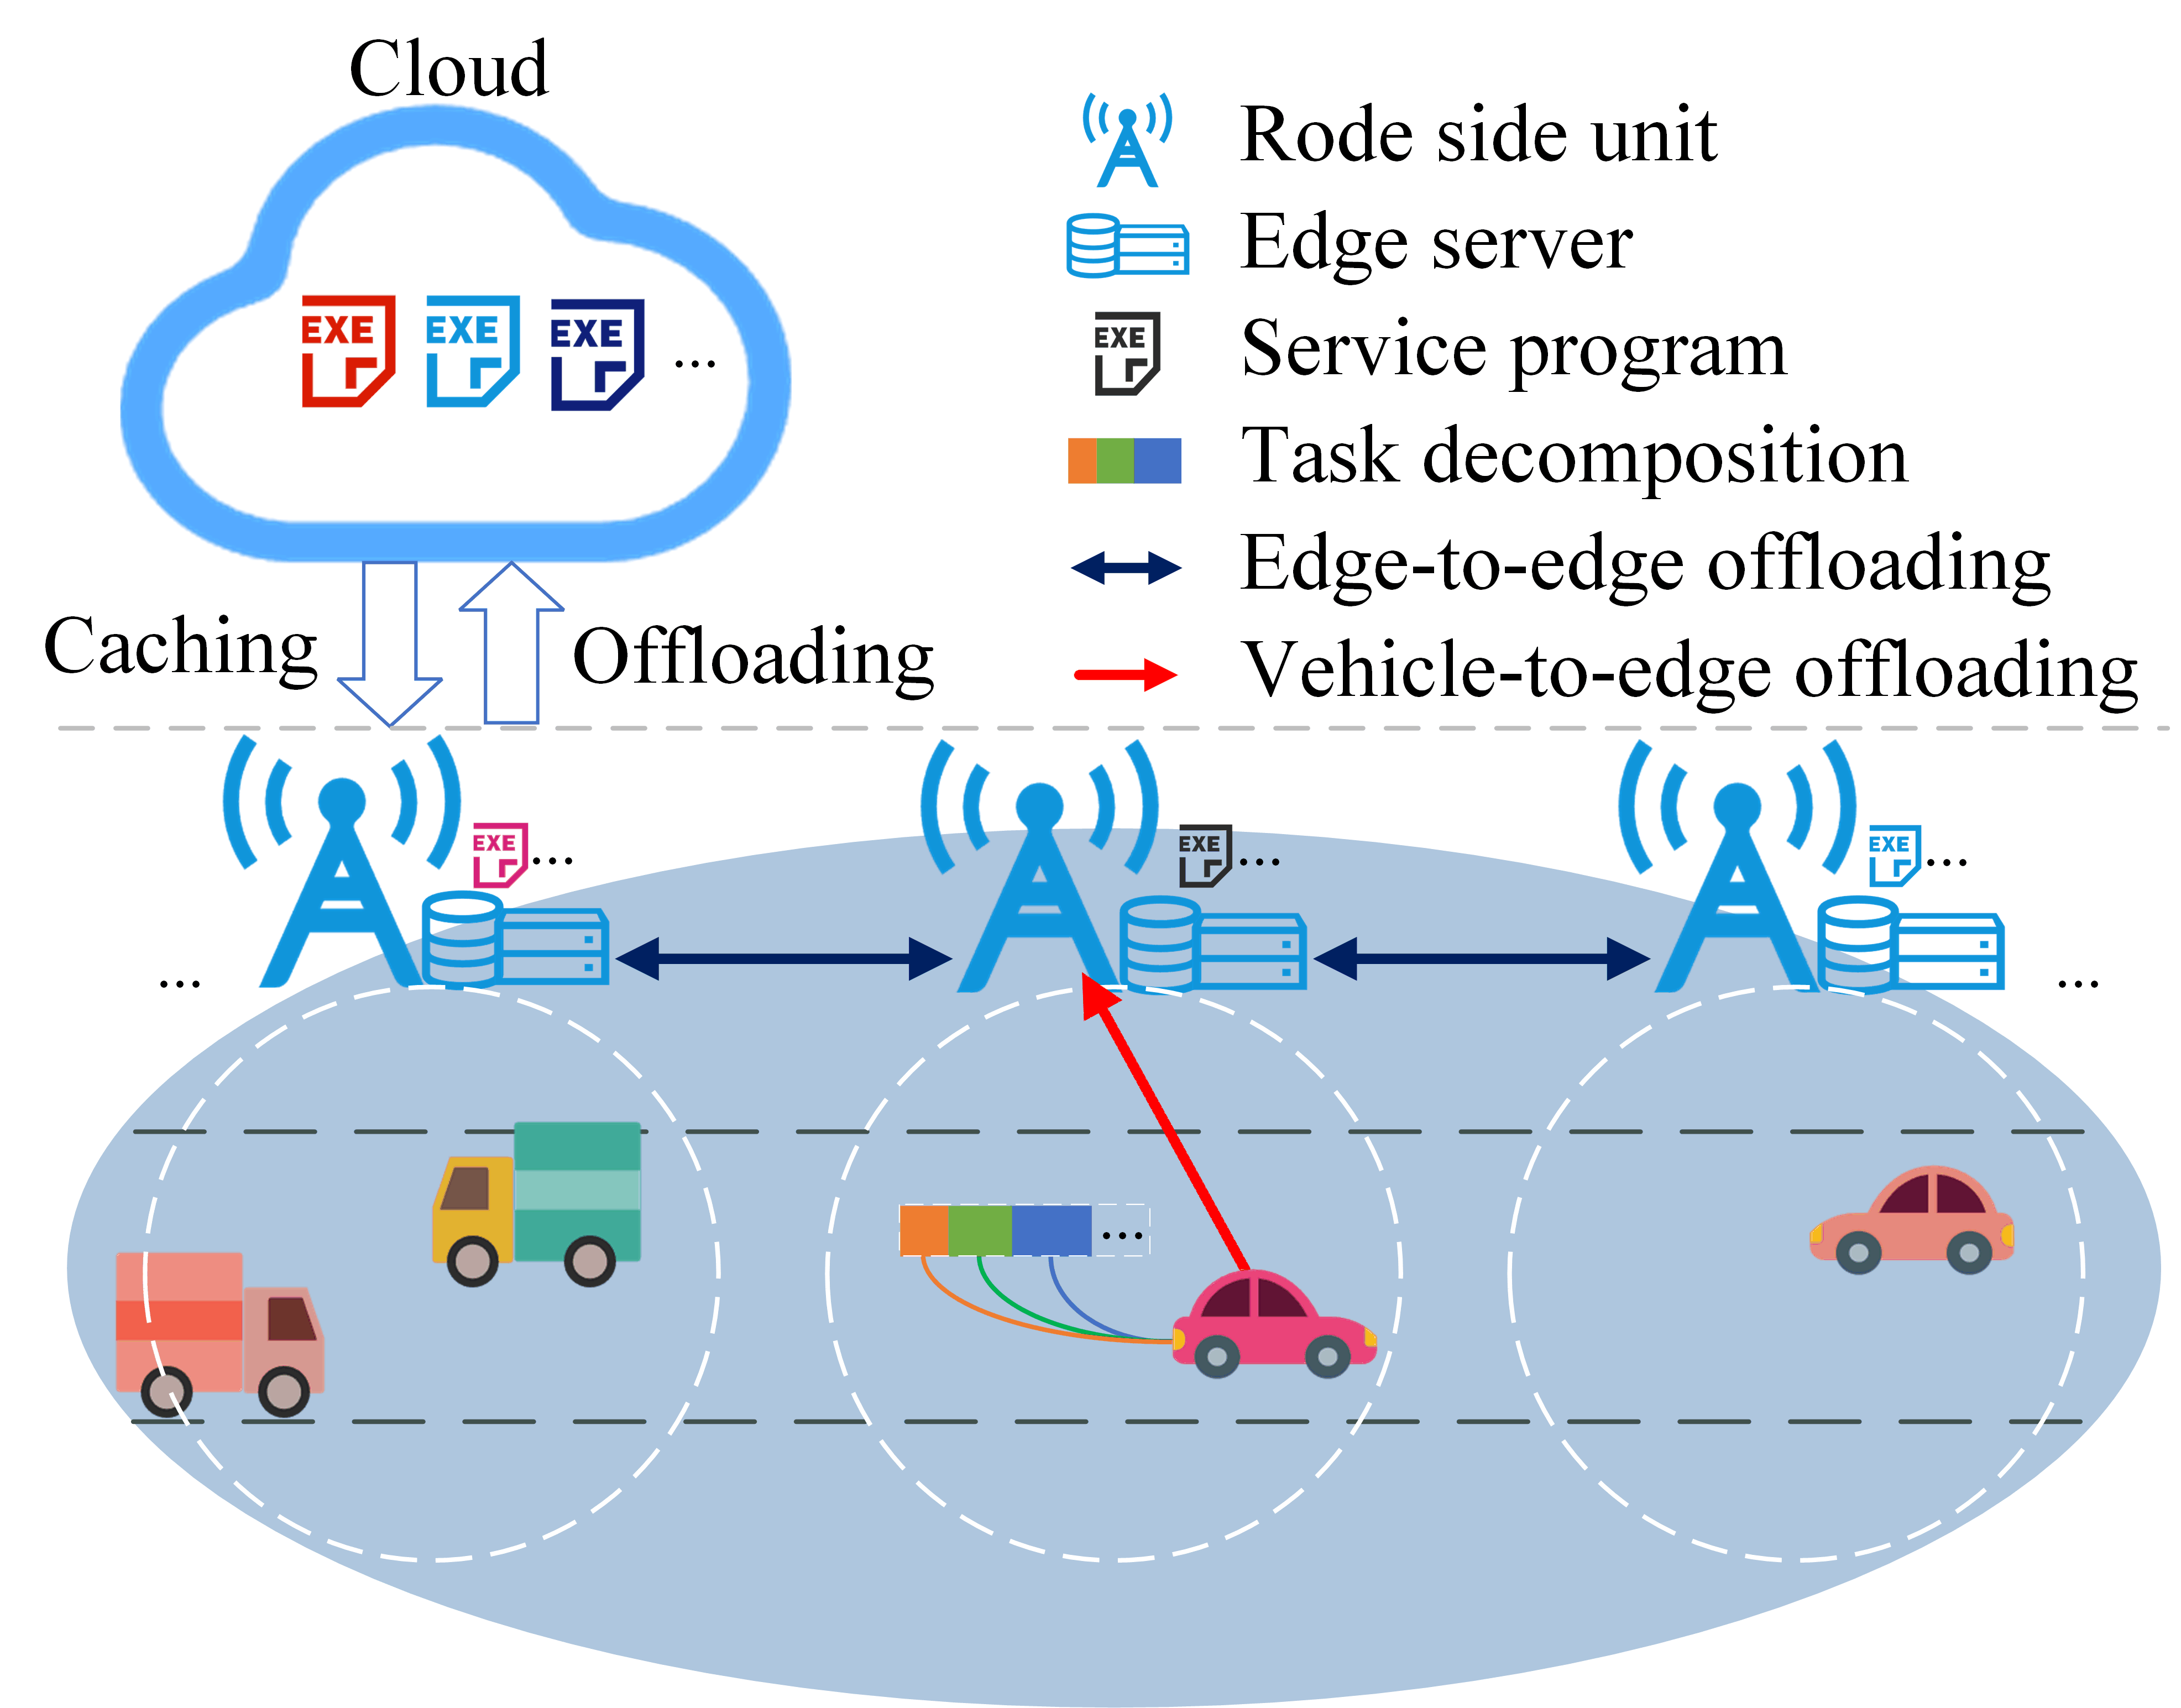
\includegraphics[width=3in]{system model.png}
	\caption{System model.}
	\label{fig: system model}
\end{figure}
% --------
The system supports $ K $ types of services, denoted by $ \mathcal{K}=\{k \mid k=1,2,\dots,K \} $, and all services are available in cloud server.
% --------
At the beginning of each time slot, the number of vehicles within the coverage area of each edge node is updated. Each vehicle generates a task that depends on multiple types of services.
During time slot $ t $, vehicle $ l $ generates a task, denoted as task $ j $.
The task $ j $ is characterized by a tuple $( d_j(t), \mathbf{f}_j(t)) $, where $ d_j(t) $ represents the input data size of task $ j $ and $  \mathbf{f}_j(t)=[ f_{j,1}(t),f_{j,2}(t),\dots,f_{j,K}(t)] \in [0,1]^{K} $ denotes the service request vector.
Specifically, $ f_{j,k}(t) $ represents the proportion of the task associated with the required service of type $ k $, satisfying 
$ \sum_{k=1}^{K}{f_{j,k}(t)}=1 $.
The effective service demand set of task $ j $ is defined as $ \mathcal{K}_{j}=\{ k | f_{j,k}>0 \} $. 
Accordingly, task $ j $  is decomposed into $ |\mathcal{K}_{j}| $ subtasks, each corresponding to a specific type of service.
For simplicity, the type $ k $ subtask of task $ j $  at time slot $ t $  is denoted as $ s_{j,k}(t) $.
Such a decomposition allows each subtask to be individually processed on an entity (vehicle,  edge node or cloud), thereby improving the overall resource utilization and flexibility of the system.

% --------
Subtasks can be processed locally on the vehicle or offloaded to the edge node that the vehicle is connected to, in order to optimize resource utilization. 
Due to the limited caching capacity, only a subset of all services can be deployed on vehicles and edge nodes.
To effectively offload tasks, each edge node considers its neighboring edge nodes as collaborative edge nodes.
% The set of collaborative edge nodes is denoted by $ \mathcal{C}_{n} = \{ m \mid m = ((n-1)\mod N) +1, ((n+1)\mod N )+1\} $.
Consequently, if neither the vehicle, the associated edge node, nor its collaborative node can fulfill  offloading requirements of the task, the task will be offloaded to the cloud server. 


% ---------------------------------------------------------------------------------------
\subsection{Communication Model} \label{Communication Model} 
This study focuses on the uplink communication scenario, where each edge node is allocated a total bandwidth of $B$, with identical bandwidth assignments across all edge nodes. With the orthogonality of the communication channels, intra-cell interference within the coverage area of a single edge node is neglected.
% At time slot $t$, the total number of tasks received by edge node $n$ is denoted by $\rho_{n}(t)$. Under these conditions, 
The signal-to-interference-plus-noise proportion (SINR) of the communication link between vehicle $l$ and edge node $n$ at time slot $t$ is given by
\begin{equation}
	\label{euq: SINR}
	\gamma_{l,n}(t) =\frac{p_{l}(t)g_{l,n}(t)}{\sum_{n=1}^{N} \left(g_{l,n}(t)\sum_{l=1}^{\rho_{n}(t)}p_{l}(t)\right) + \sigma ^2},
\end{equation}
where $p_{l}(t)$ denotes the uplink transmission power of the vehicle $ l $, $g_{l,n}(t)$ represents the average channel gain between vehicle $l$ and edge node $n$, and $\sigma^2$ is the variance of the additive white Gaussian noise. 

Based on Shannon's theorem, the data transmission rate between the vehicle $ l $ and the edge node $ n $ is given by
\begin{equation}
	\label{equ: ransimission rate}
	r_{l,n}(t) = b_{l,n}(t)\log_2( 1+\gamma_{l,n}(t) ),
\end{equation}
where $ b_{l,n}(t) = B/\rho_{n}(t) $ is the bandwidth allocated to vehicle $ l $ by edge node $ n $.






\subsection{Service Request Generation Model}
For each task, the number of required service types is sampled from a discrete distribution. 
and this reflects  that  tasks typically depend on  a few types of services. 
To model the heterogeneous service demands observed in vehicular edge computing systems, the selection of service dependencies for each task is assumed to follow by the Zipf distribution with a skewness parameter $ z>0 $ \cite{YuWu-35}. 
Specifically, the selection probability $ \mathrm{P}_{k} $  of type-$ k$ service is given by
\begin{equation}
	\label{equ: zipf}
	\mathrm{P}_{k} = \frac{\frac{1}{k^{z}}}{\sum_{k^{\prime}}^{K}{\frac{1}{{k^{\prime}}^{z}}}}.
\end{equation}

After selecting the required service types, the demand proportions for each selected service 
are assigned by a Dirichlet distribution ensuring that $ f_{j,k}(t)>0 $ and $ \sum_{k=1}^{K}{f_{j,k}(t)=1} $.
This modeling approach not only reflects the sparse and biased nature of service dependencies but also simulate  diverse task generation patterns in vehicular edge computing networks.




\subsection{Service Caching and Task Offloading Model} \label{Service Caching and Computation Offloading Model}
To fully utilize the limited caching resources of vehicles and edge nodes, we assume that each task can be processed within its originating time slot $ t $;
An agent that deployed on the cloud server determines the caching strategy for each type of service at both the vehicle and edge node  before the end of each time slot. The caching capacity constraints for the vehicle $ l $ and edge node $ n $ are given by 
\begin{equation}
	\label{equ: cache constraint 1}
	\beta \boldsymbol{\delta}^{V}_{l}(t) \cdot \mathbf{1}^{\mathrm{T}}  \le S^{V}
\end{equation}
and 
\begin{equation}
	\label{equ: cache constraint 2}
	\beta \boldsymbol{\delta}^{R}_{n}(t) \cdot \mathbf{1}^{\mathrm{T}}  \le S^{R},
\end{equation}
respectively.
% Here, the constant $ \beta $ represents the size of each service file. 
% The vectors $ \boldsymbol{\delta}^{V}_{l}(t) = [\delta^{V}_{l,1}(t), \delta^{V}_{l,2}(t), \dots, \delta^{V}_{l,K}(t)] \in \{0,1 \}^{K} $ 
% and $ \boldsymbol{\delta}^{R}_{n}(t) = [\delta^{R}_{n,1}(t), \delta^{R}_{n,2}(t), \dots, \delta^{R}_{n,K}(t)] \in \{0,1 \}^{K} $ denote the caching states of vehicle $ l $ and edge node $ n $ for all services, respectively. 
% The expression of cooperative edge's caching state is similar with $ \boldsymbol{\delta}^{R}_{n}(t) $, denoted by $ \boldsymbol{\delta}^{C}_{m}(t)=[\delta^{R}_{m,1}(t), \delta^{R}_{m,2}(t), \dots, \delta^{R}_{m,K}(t)] \in \{0,1 \}^{K} $. 
Here, the constant $ \beta $ represents the size of each service file.
The vectors $ boldsymbol{\delta}^{V}_{l}(t) $ and $ \boldsymbol{\delta}^{R}_{n}(t) $ denote the caching states of vehicle $ l $ and edge node $ n $ for all services, respectively. 
Each component of the  vector is a binary variable indicating the caching status of a specific service at an entity: a value of $ 1 $ means the service is cached, while $ 0  $ indicates it is not.
% Then, the cache hit states of vehicle $ l $ and edge node $ n $ for $ k $ type service of $ s_{j,k}(t) $  are expressed as
% \begin{equation}
% 	\label{equ: hit1}
% 	{h^{V}_{k}(t)} = 
% 		\begin{cases}
% 		1,& 			\\ 
% 		{0,}& \text{otherwise}
% 		\end{cases}
% \end{equation}
% and
% \begin{equation}
% 	\label{equ: hit2}
% 	{\delta^{R}_{n,k}(t)} = 
% 		\begin{cases}
% 		1,& \boldsymbol{\delta}^{R}_{n}(t) \ge \boldsymbol{f}_{j}(t)			\\ 
% 		{0,}& \text{otherwise}
% 		\end{cases},
% \end{equation}
% respectively.
% Similarly, the cache hit state of the collaborative edge node $ m $ is represented in the same manner as that of the edge node, denoted by $ \delta^{C}_{m,k}(t) $.

To enhance subtask execution efficiency, the agent determines the offloading destinations and proportions for all subtasks at the start of each time slot based on the cache states of all entities.
Let the continuous variables $ \omega^{V}_{l,j,k}(t) $ and $ \omega^{R}_{n,j,k}(t) $ denote the offloading proportion of subtask $ s_{j,k}(t) $  of vehicle-to-edge and edge-to-edge respectively. 
The offloading strategies corresponding to different caching deployment modes are summarized in Table~\ref{tab: caching scenarios}.
\begin{table*}[t!]
	\begin{center}
		\caption{Service deployment mode and subtask offloading proportion}
		\label{tab: caching scenarios}
		\renewcommand\arraystretch{2.5}
		\begin{tabular}{|c|c|c|c|c|c|}
				\hline
				\multicolumn{2}{|c|}{\multirow{2}{*}{Service deployment mode}} & \multicolumn{4}{c|}{Proportion offloaded to entity} 
				\\ \cline{3-6} 
				\multicolumn{2}{|c|}{} & \makecell{Vehicle $l$} & \makecell{Edge node $n$} & \makecell{Cooperative edge node $m$ } & \makecell{Cloud server} 
				\\ \hline
				{M1}
				& \makecell[c]{$\delta^{V}_{l,k}(t)=1,\delta^{R}_{n,k}(t)=0,$ \\ $\delta^{C}_{m,k}(t)\geq0$} 
				& {$1$} 
				& {$0$} 
				& {$0$} 
				& 0
				\\  \hline
				{M2} 
				& \makecell{$\delta^{V}_{l,k}(t)=1, \delta^{R}_{n,k}(t)=1,$ \\ $\delta^{C}_{m,k}(t)\geq0$}
				& {$1-\omega^{V}_{l,j,k}(t)$} 
				& {$\omega^{V}_{l,j,k}(t)$} 
				& {$0$} 
				& 0 
				\\  \hline
				{M3} 
				& \makecell{$\delta^{V}_{l,k}(t)=0, \delta^{R}_{n,k}(t)=1,$ \\ $\delta^{C}_{m,k}(t) = 0$}
				& {$0$} 
				& {$1$} 
				& {$0$} 
				& 0 
				\\  \hline
				{M4} 
				& \makecell{$\delta^{V}_{l,k}(t)=0, \delta^{R}_{n,k}(t)=1,$ \\ $\delta^{C}_{m,k}(t)=1$}
				& {$0$} 
				& {$1-\omega^{R}_{n,j,k}(t)$} 
				& {$\omega^{R}_{n,j,k}(t)$} 
				& 0 \\  \hline
				{M5} 
				& \makecell{$\delta^{V}_{l,k}(t)=0, \delta^{R}_{n,k}(t)=0,$ \\ $\delta^{C}_{m,k}(t) = 1$}
				& {$0$} 
				& {$0$} 
				& {$1$} 
				& 0 
				\\  \hline
				{M6} 
				& \makecell{$\delta^{V}_{l,k}(t)=0, \delta^{R}_{n,k}(t)=0,$ \\ $\delta^{C}_{m,k}(t)=0$}
				& {$0$} 
				& {$0$} 
				& {$0$} 
				& 1 
				\\ \hline
		\end{tabular}
	\end{center}
\end{table*}


Specifically, the agent performs fine-grained subtask offloading for each task. For the type-$k$ service required by subtask $s_{j,k}(t)$, it first checks whether the service is cached locally. If so, the agent further verifies whether the associated edge node $n$ also caches the service, to determine whether the subtask should be fully executed locally  or partially offloaded to a edge node.
If the service is not cached at the vehicle, the subtask is fully uploaded to the associated edge node $n$. Based on the caching states of edge node $n$ and its cooperative edge nodes, the agent then decides whether to offload the entire subtask to node $n$, to a cooperative node, or partially to both.
It is worth noting that when multiple cooperative edge nodes meet the subtask offloading requirements, one of them is randomly selected for collaboration.
If neither the vehicle, the edge node, nor the cooperative edge nodes cache the type-$ k $ service, the subtask is offloaded to the cloud server.
The detailed offloading procedure is illustrated in Fig. \ref{fig: flowchart}.
\begin{figure*}[!t]
	\centering
	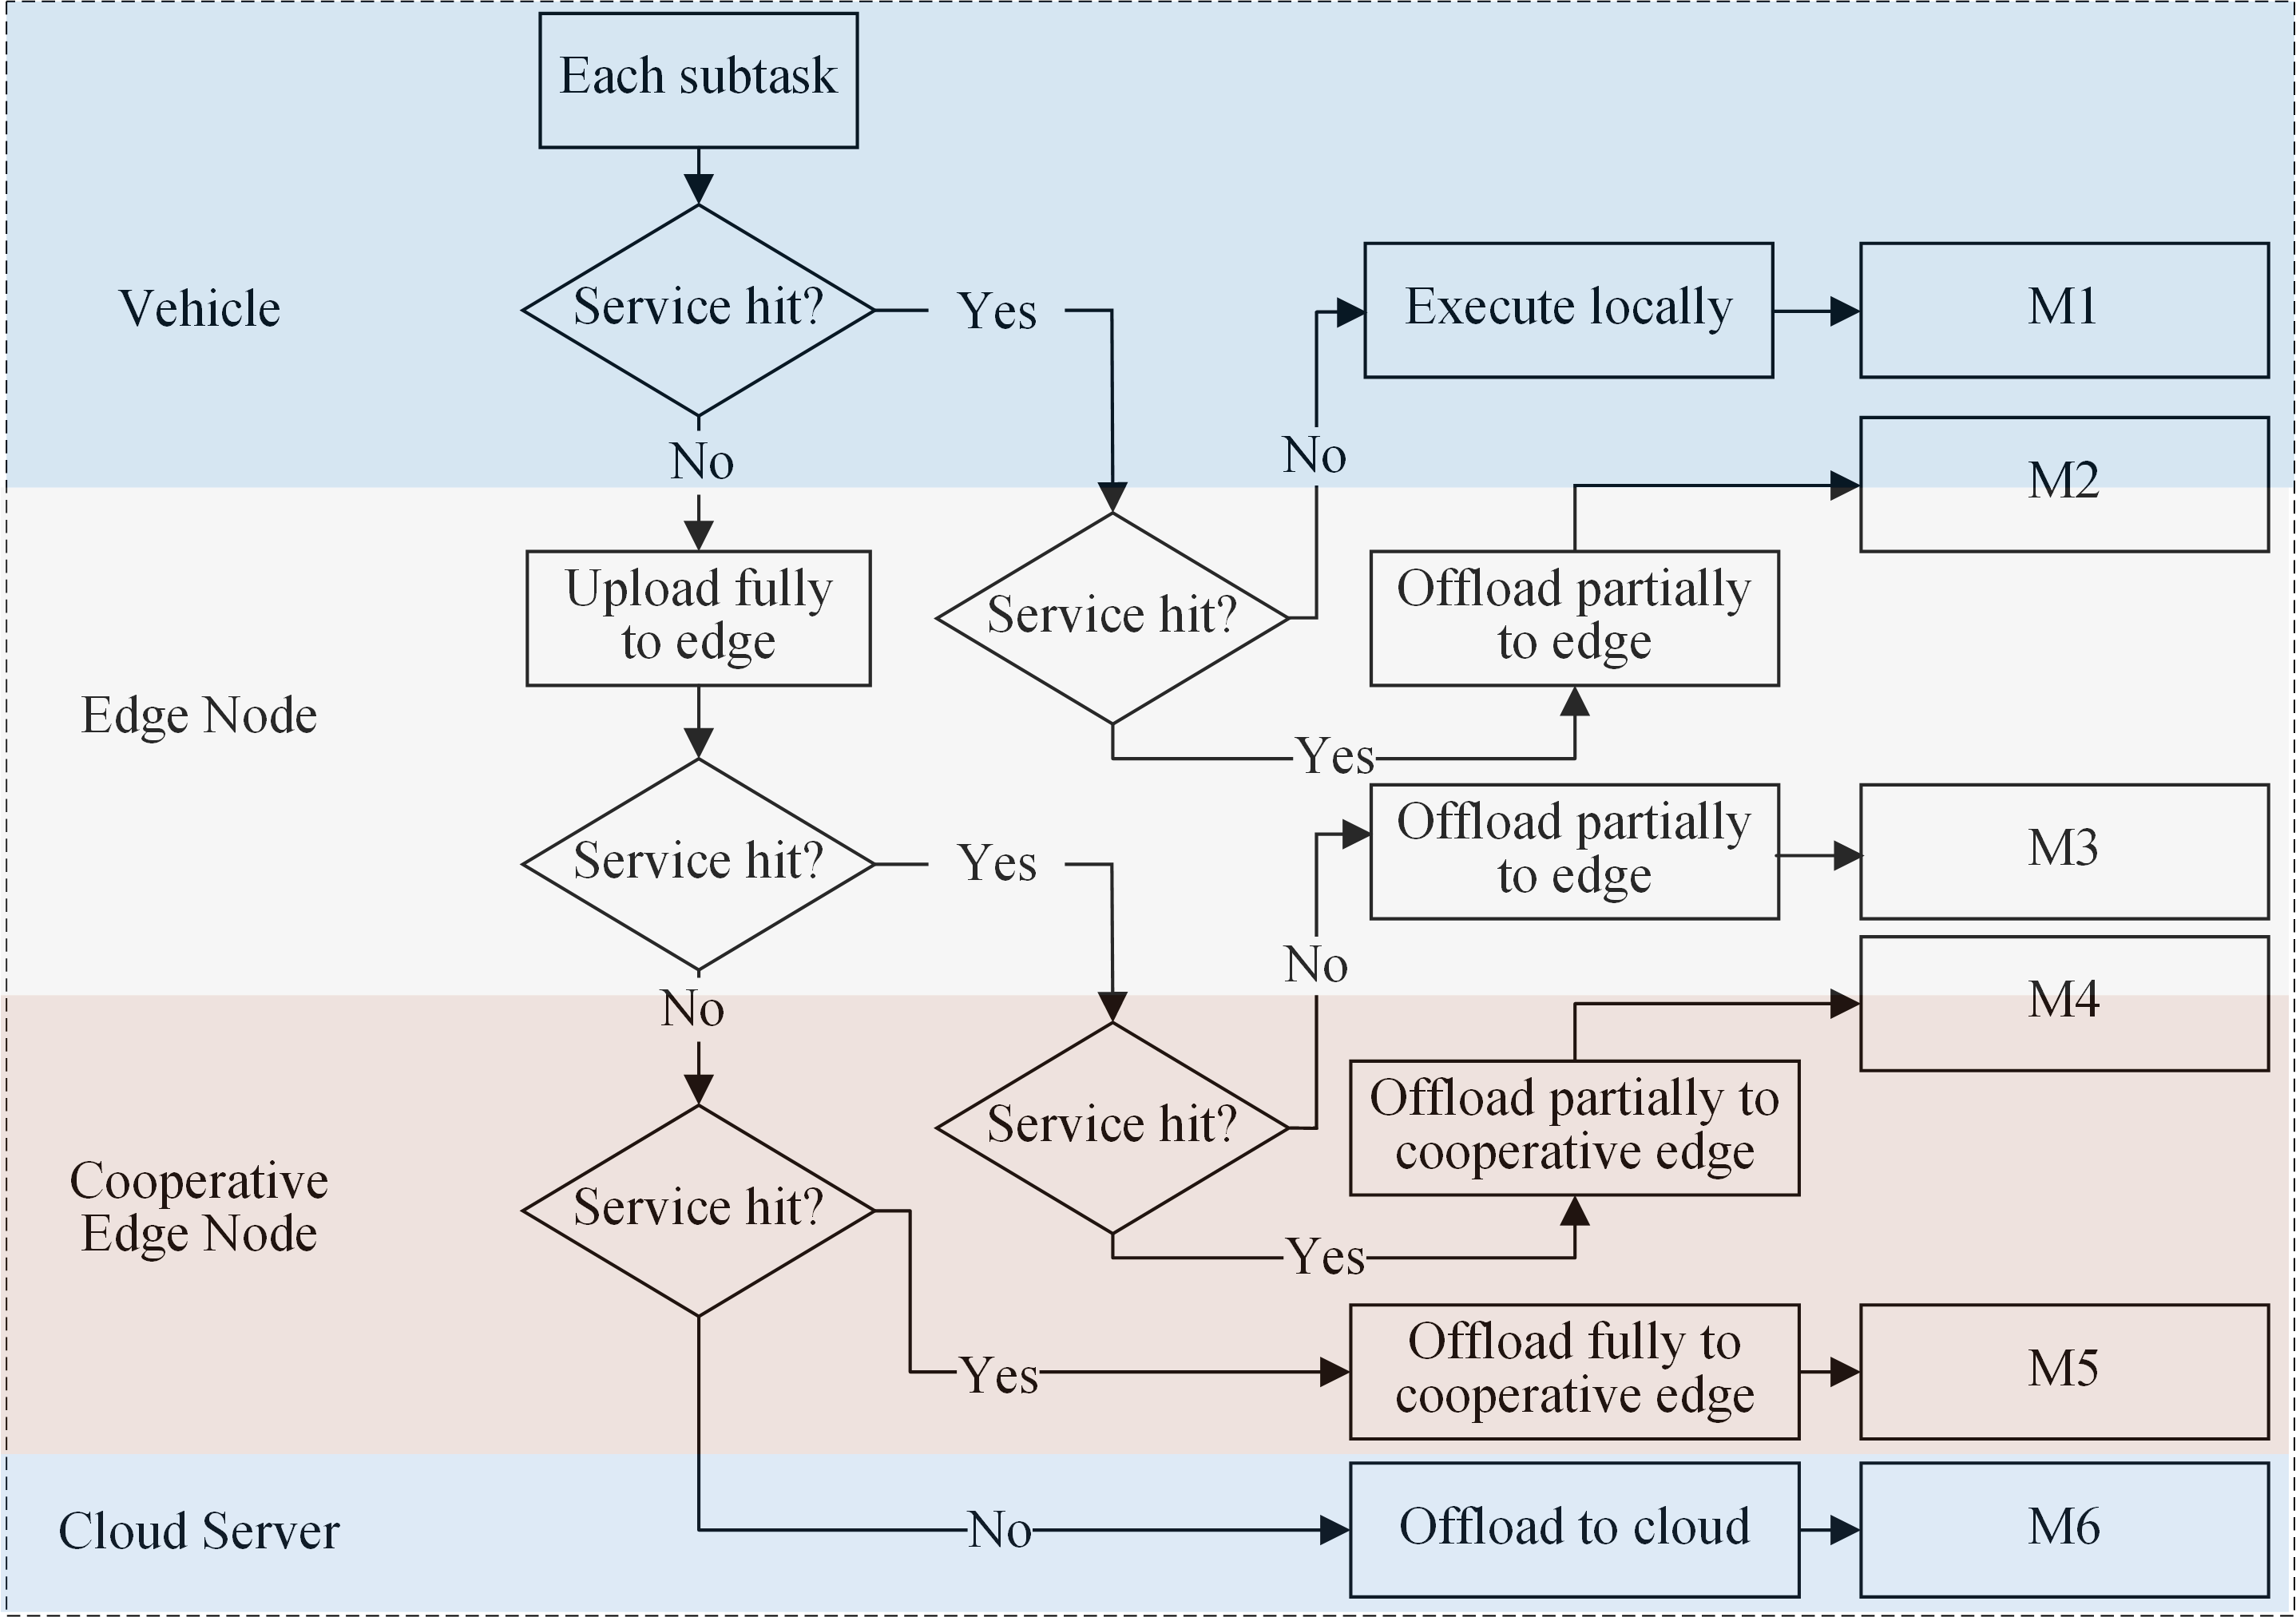
\includegraphics[width=6in]{flowchart}
	\caption{Flowchart of  offloading.}
	\label{fig: flowchart}
\end{figure*}

\subsection{Computation Delay and Energy Consumption}
\label{Computation Delay and Energy Consumption}
Based on Sec. \ref{Communication Model} and Sec. \ref{Service Caching and Computation Offloading Model}, the delay of subtask $ s_{j,k}(t) $ is calculated as follows. 

The computation delay locally is given by
\begin{equation}
	\label{equ: local delay}
	D^{local}_{l,j,k}(t) = \delta^{V}_{l,k}(t)(1-\omega^{V}_{l,j,k}(t)) \frac{\lambda d_{j,k}(t)}{f^{V}},
\end{equation}
where $f^{V}$ represents the CPU frequency of a vehicle, and $\lambda$ denotes the number of CPU cycles required to compute one bit of data. If the subtask is offloaded to edge node $n$, the transmission delay for uploading the input data is given by
\begin{equation}
	\label{equ: uploaded to edge node delay}
	D_{l,j,k}^{up}(t) = \left( 1-\delta^{V}_{l,k}(t)(1-\delta^{R}_{n,k}(t)) \right) \omega^{V}_{l,j,k}(t)\frac{d_{j,k}(t)}{r_{l,n}(t)}.
\end{equation}
The computation delay at edge node $ n $ is expressed as 
\begin{equation}
	\label{equ: edge node delay}
	D^{edge}_{n,j,k}(t) = \delta^{R}_{n,k}(t)\omega^{V}_{l,j,k}(t)(1-\omega^{R}_{n,j,k}(t))\frac{\lambda d_{j,k}(t)}{f^{R}},
\end{equation}
where $f^{R}$ denotes the CPU frequency of the edge server. If the subtask is further offloaded from edge node $n$ to a cooperative edge node $m$, the transmission delay between edge nodes can be expressed as
\begin{equation}
	\label{equ: uploaded to coo edge delay}
	D_{n,j,k}^{e2e}(t) =(1-\delta^{V}_{l,k}(t))\delta^{C}_{m,k}(t)\omega^{V}_{l,j,k}(t)\omega^{R}_{n,j,k}(t)\frac{d_{j,k}(t)}{r^{e2e}},
\end{equation}
where $ r^{e2e} $ represents the data transmission rate between edge nodes.
The computation delay at the cooperative edge node $ m $ is expressed as 
\begin{equation}
	\label{coopertate edge delay}
	D^{co}_{m,j,k}(t) = (1-\delta^{V}_{l,k}(t))\delta^{C}_{m,k}(t)\omega^{V}_{l,j,k}(t)\omega^{R}_{n,j,k}(t)\frac{\lambda d_{j,k}(t)}{f^{R}}.
\end{equation}
If the vehicle $l$, edge node $n$, and cooperative edge node $m$ do not meet the offloading conditions, the subtask will be uploaded from the edge node $ n $ to the cloud server, with the transmission delay given by
\begin{equation}
	\label{equ: cloud delay}
	D^{cloud}_{n,j,k}(t) = \left( 1-\left( \delta^{V}_{l,k}(t) + \delta^{R}_{n,k}(t) +\delta^{C}_{m,k}(t) \right) \right) \frac{d_{j,k}(t)}{r^{e2c}}
\end{equation}
where $ r^{e2c} $ denotes the data transmission rate from edge node to remote cloud server. 
In the delay calculations above, since the task output is much smaller than the input and the cloud server has substantial computational resources, the delay caused by result transmission and cloud computation is negligible \cite{JJWu}.  
In summary, the execution delay of the subtask $ s_{j,k}(t) $ can be expressed as:
\begin{equation}
	\label{equ: subtask delay}
	\begin{aligned}
		D_{j,k}^{total}(t) = & \max \Bigg \{ D^{local}_{l,j,k}(t), D^{up}_{l,j,k}(t) + \max \Big\{D^{edge}_{n,j,k}(t),  \\
		&   D^{e2e}_{n,j,k}(t)+D^{co}_{m,j,k}(t),  D^{cloud}_{n,j,k}(t)\Big\} \Bigg\}, 
	\end{aligned}
\end{equation}
which encompasses all the service deployment modes presented in Table \ref{tab: caching scenarios}. 
Then the execution delay of task $ j $ is defined as
\begin{equation}
	\label{equ: total delay}
	D_{j}^{total}(t) = \sum_{k \in \mathcal{K}_j}{D_{j,k}^{total}(t)}.
\end{equation}
The average delay for executing all tasks in the system at time slot $ t $ is defined as follows
\begin{equation}
	\label{equ: average delay}
	D^{ave}(t) = \frac{1}{N} \sum_{n=1}^{N} \left( \frac{1}{\rho_{n}(t)} \sum_{i=1}^{\rho_{n}(t)} D_{j}^{total}(t) \right).
\end{equation}
According to \cite{KongDuan-10}, the MNOs' energy consumption is considered in our study, which includes the energy consumption by edge servers and cloud servers. The total energy consumption for executing subtask $ s_{j,k}(t) $ is given as follows.
\begin{equation}
	\label{equ: subtask energy consumption}
	\begin{aligned}
		E_{j,k}^{total}(t) = & \kappa (f^{R})^2 \left( D^{edge}_{n,j,k}(t)+D^{co}_{m,j,k}(t) \right)  \\
		+ & p^{e2e} D_{n,j,k}^{e2e} + p^{e2c} D^{cloud}_{n,j,k}(t).
	\end{aligned}
\end{equation}
Here,  $ \kappa $ represents the processor energy efficiency parameter of edge server, which typically depends on hardware conditions. Parameters $ p^{e2e} $ and  $ p^{e2c} $ denote the edge-to-edge transmit power and  edge-to-cloud transmit power, respectively.  
Then the execution energy consumption of task $ j $ is defined as
\begin{equation}
	\label{equ: total energy consumption}
	E_{j}^{total}(t) = \sum_{k \in \mathcal{K}_j}{E_{j,k}^{total}(t)}.
\end{equation}
The average energy consumption is similar with \eqref{equ: average delay}, defined as
\begin{equation}
	\label{average energy consumption}
	E^{ave}(t) = \frac{1}{N} \sum_{n=1}^{N} \left( \frac{1}{\rho_{n}(t)} \sum_{i=1}^{\rho_{n}(t)} E_{j}^{total}(t) \right).
\end{equation}


\subsection{Computation Delay and Energy Consumption Extremum Analysis}
In the Sec. \ref{Computation Delay and Energy Consumption}, the delay and energy consumption was conducted from the perspective of subtask offloading flow. 
In this section, we further evaluate the delay and energy consumption under different service deployment modes and derive extremum values, which helps to understand the best-case and worst-case performance of subtask offloading and reveal the performance boundaries caused by different caching conditions.

The execution delay and MNOs' energy consumption  of for subtask $ s_{j,k}(t) $ in different modes is as follows:
\begin{enumerate}
	\item
	M1: The subtask is computed locally 
	\begin{equation}
		\label{equ: M1}
		D^{M1}(t)= \frac{\lambda d_{j,k}(t)}{f^{V}},
	\end{equation}
	\begin{equation}
		E^{M1}(t) = 0.
   \end{equation}
	\item 
	M2: A part of the subtask is computed locally, and the remaining part is offloaded to edge node
	\begin{equation}
		\label{equ: M2}
		\begin{aligned}
			D^{M2}(t)=& \max \Bigg\{(1-\omega^{V}_{l,j,k}(t)) D^{M1} , \\
			&\omega^{V}_{l,j,k}(t)\left( \frac{d_{j,k}(t)}{r_{l,n}(t)} +\frac{\lambda d_{j,k}(t)}{f^{R}}  \right)\Bigg\},
		\end{aligned}
	\end{equation} 
	\begin{equation}
		E^{M2}(t) = \kappa f^{R} \omega^{V}_{l,j,k}(t) \lambda d_{j,k}(t).
	\end{equation}
	\item
	M3: The subtask is fully offloaded to edge node
	\begin{equation}
		\label{equ: M3}
		D^{M3}(t)=  \frac{d_{j,k}(t)}{r_{l,n}(t)} +\frac{\lambda d_{j,k}(t)}{f^{R}},
	\end{equation}
	\begin{equation}
		E^{M3}(t) = \kappa f^{R} \lambda d_{j,k}(t).
	\end{equation}
	\item
	M4: The subtask is offloaded to both  edge node and cooperative edge node 
	\begin{equation}
		\label{equ: M4}
		\begin{aligned}
			D^{M4}(t)=  & \frac{d_{j,k}(t)}{r_{l,n}(t)}+ \max\Bigg\{ \frac{(1-\omega^{R}_{n,j,k}(t)) \lambda d_{j,k}(t)}{f^{R}}, \\
						& \omega^{R}_{n,j,k}(t)\left(   \frac{d_{j,k}(t)}{r^{e2e}} +  \frac{\lambda d_{j,k}(t)}{f^{R}} \right) \Bigg\}.
		\end{aligned}
	\end{equation}
	\begin{equation}
		E^{M4}(t) = \kappa f^{R} \lambda d_{j,k}(t) + \omega_{n,j,k}^{R}(t) p^{e2e} \frac{d_{j,k}(t)}{r^{e2e}},
	\end{equation}
	\item 
	M5: The subtask is fully offloaded to  cooperative edge node 
	\begin{equation}
		\label{equ: M5}
		D^{M5}(t)=  \frac{d_{j,k}(t)}{r_{l,n}(t)} + \frac{d_{j,k}(t)}{r^{e2e}} +\frac{\lambda d_{j,k}(t)}{f^{R}},
	\end{equation}
	\begin{equation}
		E^{M5}(t) = \kappa f^{R} \lambda d_{j,k}(t) +p^{e2e} \frac{d_{j,k}(t)}{r^{e2e}}.
	\end{equation}
	\item
	M6: The task is fully offloaded to cloud server
	\begin{equation}
		\label{equ: M6}
		D^{M6}(t)= \frac{d_{j,k}(t)}{r_{l,n}(t)}+ \frac{d_{j,k}(t)}{r^{e2c}},
	\end{equation}
	\begin{equation}
		E^{M6}(t) = p^{e2c} \frac{d_{j,k}(t)}{r^{e2c}}.
	\end{equation}
\end{enumerate}
By comparing the execution delay under different service deployment modes, the maximum value  can be derived as
\begin{equation}
	\label{equ: max delay}
	\max\{D_{j,k}^{total}(t)\} = \max\{ D^{M1}(t), D^{M5}(t), D^{M6}(t) \},
\end{equation}
and the minimum value can be derived as
\begin{equation}
	\min\{D_{j,k}^{total}(t)\} = \min\{D^{M2}(t), D^{M4}(t), D^{M6}(t)\}.
\end{equation}
According to convex piecewise optimization, the offloading proportion of \eqref{equ: M2} and \eqref{equ: M4} can be eliminated, i.e., when  $ \omega^{V}_{l,j,k}(t) $ takes the following value
\begin{equation}
	\omega^{V}_{l,j,k}(t) = \frac{1}{(1+\frac{f^{V}}{\lambda r_{l,n}(t)}+\frac{f^{V}}{f^{R}})}, 
\end{equation}
the minimum value of $ D^{M2}(t) $ can be expressed as
\begin{equation}
	\min\{ D^{M2}(t) \} = \frac{ \lambda d_{j,k}(t) \left( f^{R} + \lambda r_{l,n}(t) \right) }{ \lambda f^{R} f^{V} + f^{R} r_{l,n}(t) + \lambda r_{l,n}(t) f^{V} },
\end{equation}
and the minimum value of $ D^{M4}(t) $ can be expressed as
\begin{equation}
	\min\{ D^{M4}(t) \} = \frac{d_{j,k}(t)}{r_{l,n}(t)} + \frac{ \lambda d_{j,k}(t) \left( f^{R} + \lambda r^{e2e} \right) }{ f^{R} \left( f^{R} + 2\lambda r^{e2e} \right) },
\end{equation}
when $ \omega^{R}_{n,j,k}(t) $ takes the following value
\begin{equation}
	\omega^{R}_{n,j,k}(t) = \frac{1}{(2+ \frac{f^{R}}{\lambda r^{e2e}} )}.
\end{equation}
Hence, the minimum value of the execution delay can be also expressed as 
\begin{equation}
	\label{equ: min delay}
	\begin{aligned}
		\min\{D_{j,k}^{total}(t)\} =& \min \Big\{\min\{D^{M2}(t)\}, \min\{D^{M4}(t)\}, \\
		& D^{M6}(t) \Big\}.
	\end{aligned}
\end{equation}

From the energy consumption analysis under different modes, the minimum energy consumption incurred by MNOs for subtask execution is $0 $, while the maximum energy consumption is represented as
\begin{equation}
	\label{equ: max energy}
	\max\{ E^{total}_{j,k}(t) \} =\max \left\{ E^{M5}(t),E^{M6}(t) \right\}.
\end{equation}

According to \eqref{equ: max delay} and \eqref{equ: min delay}, the subtask execution delay is closely related to factors such as subtask data size and device computing capabilities. The maximum delay may occur in M1, M5 or M6, while the minimum delay is likely to occur in M2, M4, or M6. 
The reason why M6 appears in both the maximum and minimum delay cases is that, when a subtask is offloaded to the cloud server, the delay is highly sensitive to the data size. Once the data size exceeds a certain threshold, the maximum delay tends to occur in M6.
This suggests that to minimize execution delay, the agent should involve edge nodes in subtask computation as much as possible, i.e., prioritize caching services at the edge nodes.  
Meanwhile, \eqref{equ: max energy} shows that the maximum energy consumption arises in  M5 or M6. Although the participation of edge nodes increases energy consumption, if the agent can realize more service deployment modes M2 and M4, it will effectively reduce the delay while keeping MNOs' energy consumption within a reasonable range. 

Deriving the extremum values of execution delay and energy consumption offers guidance for the design of subsequent scheme design such the parameter setting in simulation experiments and informs the  optimization direction by clarifying the effects of service availability on offloading decisions. 





\subsection{Problem Formulation} 
In this section, to minimize the long-term cumulative average latency, the problem of service caching and task offloading is formulated as a MINLP optimization problem. Let $ \mathbf{Z}(t) $ denote decision variables at time slot  $ t $, i.e., $  \mathbf{Z}(t) = [ \omega^{V}_{l,j,k}(t), \omega^{R}_{n,j,k}(t), \delta^{V}_{l,k}(t),\delta^{R}_{n,k}(t)] $.  
The detailed problem formulation is presented as follows.
\begin{align}
	% \{ \omega^{V}_{l,j,k}(t), \omega^{R}_{n,j,k}(t), \delta^{V}_{l,k}(t),\delta^{R}_{n,k}(t) \}
	% \label{equ: problem formulation}
		&\underset{\mathbf{Z}(t)}{\min} \quad \sum_{t=0}^{T-1} D^{\text{ave}}(t),
		\label{equ: PF}
		\\
		& \text{s.t.} \notag
		\\
		& \forall l\in \mathcal{L}, \forall n\in \mathcal{N}, \forall k\in \mathcal{K}, \forall t\in \mathcal{T}, \notag
		\\
		& \omega^{V}_{l,j,k}(t)\in [0,1], 
		\tag{\ref{equ: PF}a}
		\label{a} 
		\\
		&\omega^{R}_{n,j,k}(t)\in [0,1], 
		% \forall m\in\mathcal{C}_n,n,t,
		\tag{\ref{equ: PF}b}
		\label{b} 
		\\
		&\omega^{V}_{l,j,k}(t) + \omega^{R}_{n,j,k}(t)=1
		\tag{\ref{equ: PF}c}
		\label{c} 
		\\
		&\delta^{V}_{l,k}(t)\in \{0,1\}, 
		% \forall k\in \mathcal{K},l,t ,
		\tag{\ref{equ: PF}d}
		\label{d} 
		\\
		&\delta^{R}_{n,k}(t)\in \{0,1\}, 
		% \forall n,k,t ,
		\tag{\ref{equ: PF}e}
		\label{e} 
		\\
		&\beta \boldsymbol{\delta}^{V}_{l}(t) \cdot \mathbf{1}^{\mathrm{T}}  \le S^{V}, 
		% \forall l,k,t ,
		\tag{\ref{equ: PF}f}
		\label{f} 
		\\
		&\beta \boldsymbol{\delta}^{R}_{n}(t) \cdot \mathbf{1}^{\mathrm{T}}  \le S^{R}.
		% \forall n,k,t.
		\tag{\ref{equ: PF}g}
		\label{g} 
\end{align}
In \eqref{equ: PF}, 
constraints \eqref{a}, \eqref{b} and \eqref{c} ensure that the offloading ratios of a subtask are continuous values within the range $ [0,1] $ and sum to one, thereby guaranteeing the completeness of task offloading;  
constraints \eqref{d} and \eqref{e} specify that the caching states of a particular service at a vehicle or edge node is represented by binary variables;  
constraints \eqref{f} and \eqref{g} ensure that the cached services do not exceed the storage capacity of vehicles or edge nodes.

\section{The Proposed DRLSCCO Scheme}
Traditional methods, such as convex optimization and game theory, are commonly used in edge computing but struggle in the dynamic VEC environment due to their static nature. Heuristic and rule-based algorithms, though computationally feasible, fail to generalize across varying VEC scenarios.  
The DDPG algorithm, a DRL algorithm combining deep neural networks (DNN) and reinforcement learning (RL), enables agents to interact with the environment and make decisions based on experiences, especially suited for high-dimensional systems like VEC, where continuous decision variables such as offloading proportion are involved \cite{DavidGuy-22}. 
In this section, we transform the problem in \eqref{equ: PF} as a Markov Decision Process (MDP) and propose a DDPG-based joint service caching and computation offloading scheme, DRLSCCO, to optimize caching and offloading decisions, with a detailed explanation of the DRLSCCO scheme.




\subsection{Problem Formulation Based on RL}
In the proposed DRLSCCO scheme, the DDPG algorithm operates within RL framework, which is typically formulated as  MDP. The MDP leverages the Markov property, where future state transitions depend solely on the current state, independent of past states.  
We first transform the problem as an MDP, providing a formal structure for sequential decision-making in stochastic VEC environments, allowing the agent to learn  policies through interaction with the system over time.  
A typic MDP consists of three key elements: a state space $ \mathbf{S} $ representing system conditions, an action space  $ \mathbf{A} $  defining  decisions, and a reward function  $ r $ that evaluates actions and guides learning. These three elements are defined as follows:
\subsubsection{State space}
According to the proposed system model, the system state includes the following components:
\begin{itemize}
	\item $ \boldsymbol{\delta}^{\text{V}}(t) $: The caching state of vehicles for services at time slot $ t $.
	\item $ \boldsymbol{\delta}^{\text{R}}(t) $: The caching state of edge nodes for services at time slot $ t $.
	\item $ \mathbf{d}(t) $: The task size generated by vehicles at time slot $ t $.
	\item $ \mathbf{b}(t) $: The bandwidth allocated to vehicles at time slot $ t $.
	\item $ \boldsymbol{\gamma}(t) $: The received SINR of edge nodes when communicating with vehicles at time slot $ t $.
\end{itemize}
At the beginning of the time slot $ t $, the state space of system can be expressed as
\begin{equation}
	\label{equ: state space}
	\begin{aligned}
		\mathbf{S}(t) =  & \left\{ [\boldsymbol{\delta}^{\text{V}}(t)]^{ L \times K},  [\boldsymbol{\delta}^{\text{R}}(t)]^{N \times K},[\mathbf{d}(t)]^{L},  \right.  \\ 
		  & \left.  [\mathbf{b}(t)]^{ L}, [\boldsymbol{\gamma}(t)]^{L} \right\}.
	\end{aligned}
\end{equation}
% To simplify state representation, the state space $ \mathbf{S}(t) $ can be mapped to one-dimensional scalar state $ s_t $.
\subsubsection{Action space}
After obtaining the system state, the agent determines the subtask offloading locations and offloading proportion before the end of time slot, while also updating the  service deployment of vehicles and edge nodes. The action space  at time slot $ t $ includes the following components:
\begin{itemize}
	\item $ \boldsymbol{\delta}^{\text{V}}(t) $: The caching decisions of vehicles for  services at time slot $ t $.
	\item $ \boldsymbol{\delta}^{\text{R}}(t)$: The caching decisions of edge nodes for all services at time slot $ t $.
	\item $\boldsymbol{\omega}^{\text{V}}(t) $: The proportion of  tasks offloaded to  connected edge node at time slot $ t $.
	\item $\boldsymbol{\omega}^{\text{R}}(t)$: The proportion of  tasks transmitted from an edge node to a cooperative edge node at time slot $ t $.
\end{itemize}
The action space at time slot $ t $ can be represented as
\begin{equation}
	\label{equ: action space}
	\begin{aligned}
		\mathbf{A}(t) = & \left\{  [\boldsymbol{\delta}^{\text{V}}(t)]^{\times L \times K},   [\boldsymbol{\delta}^{\text{R}}(t)]^{N \times K} \right. \\
						& \left. [ \boldsymbol{\omega}^{\text{V}}(t)]^{ L},  [ \boldsymbol{\omega}^{\text{R}}(t)]^{L}         \right\}.
	\end{aligned}
\end{equation}
% which can be mapped to one-dimensional scalar state $ a_t $.
\subsubsection{Reward}
The reward in RL provides immediate feedback on the agent's actions, guiding its decision-making by evaluating the quality of decisions in a given state and influencing future behavior.
Given a state $ \mathbf{S}(t) $ and action $ \mathbf{A}(t) $, the reward at time slot $ t $ is defined as  
\begin{equation}
	\label{equ: reward}
	r_t = r(\mathbf{S}(t),\mathbf{A}(t)) = -D^{ave}(t).
\end{equation}

\subsection{DDPG-Based Service Caching and Task offloading Scheme}
At each time slot, the environment is characterized by the state space $ \mathbf{S}(t) $  and the action space $ \mathbf{A}(t) $, which describe all possible states and actions.
The agent's  policy is continuously updated through iterative interactions with the environment, gradually converging to an optimal strategy. The agent architecture in DRLSCCO—comprising policy and target networks as well as a replay buffer—is designed to support this learning process. The framework of the DRLSCCO scheme is illustrated in Fig. \ref{fig: DRLSCCO}.
\begin{figure}[!t]
	\centering
	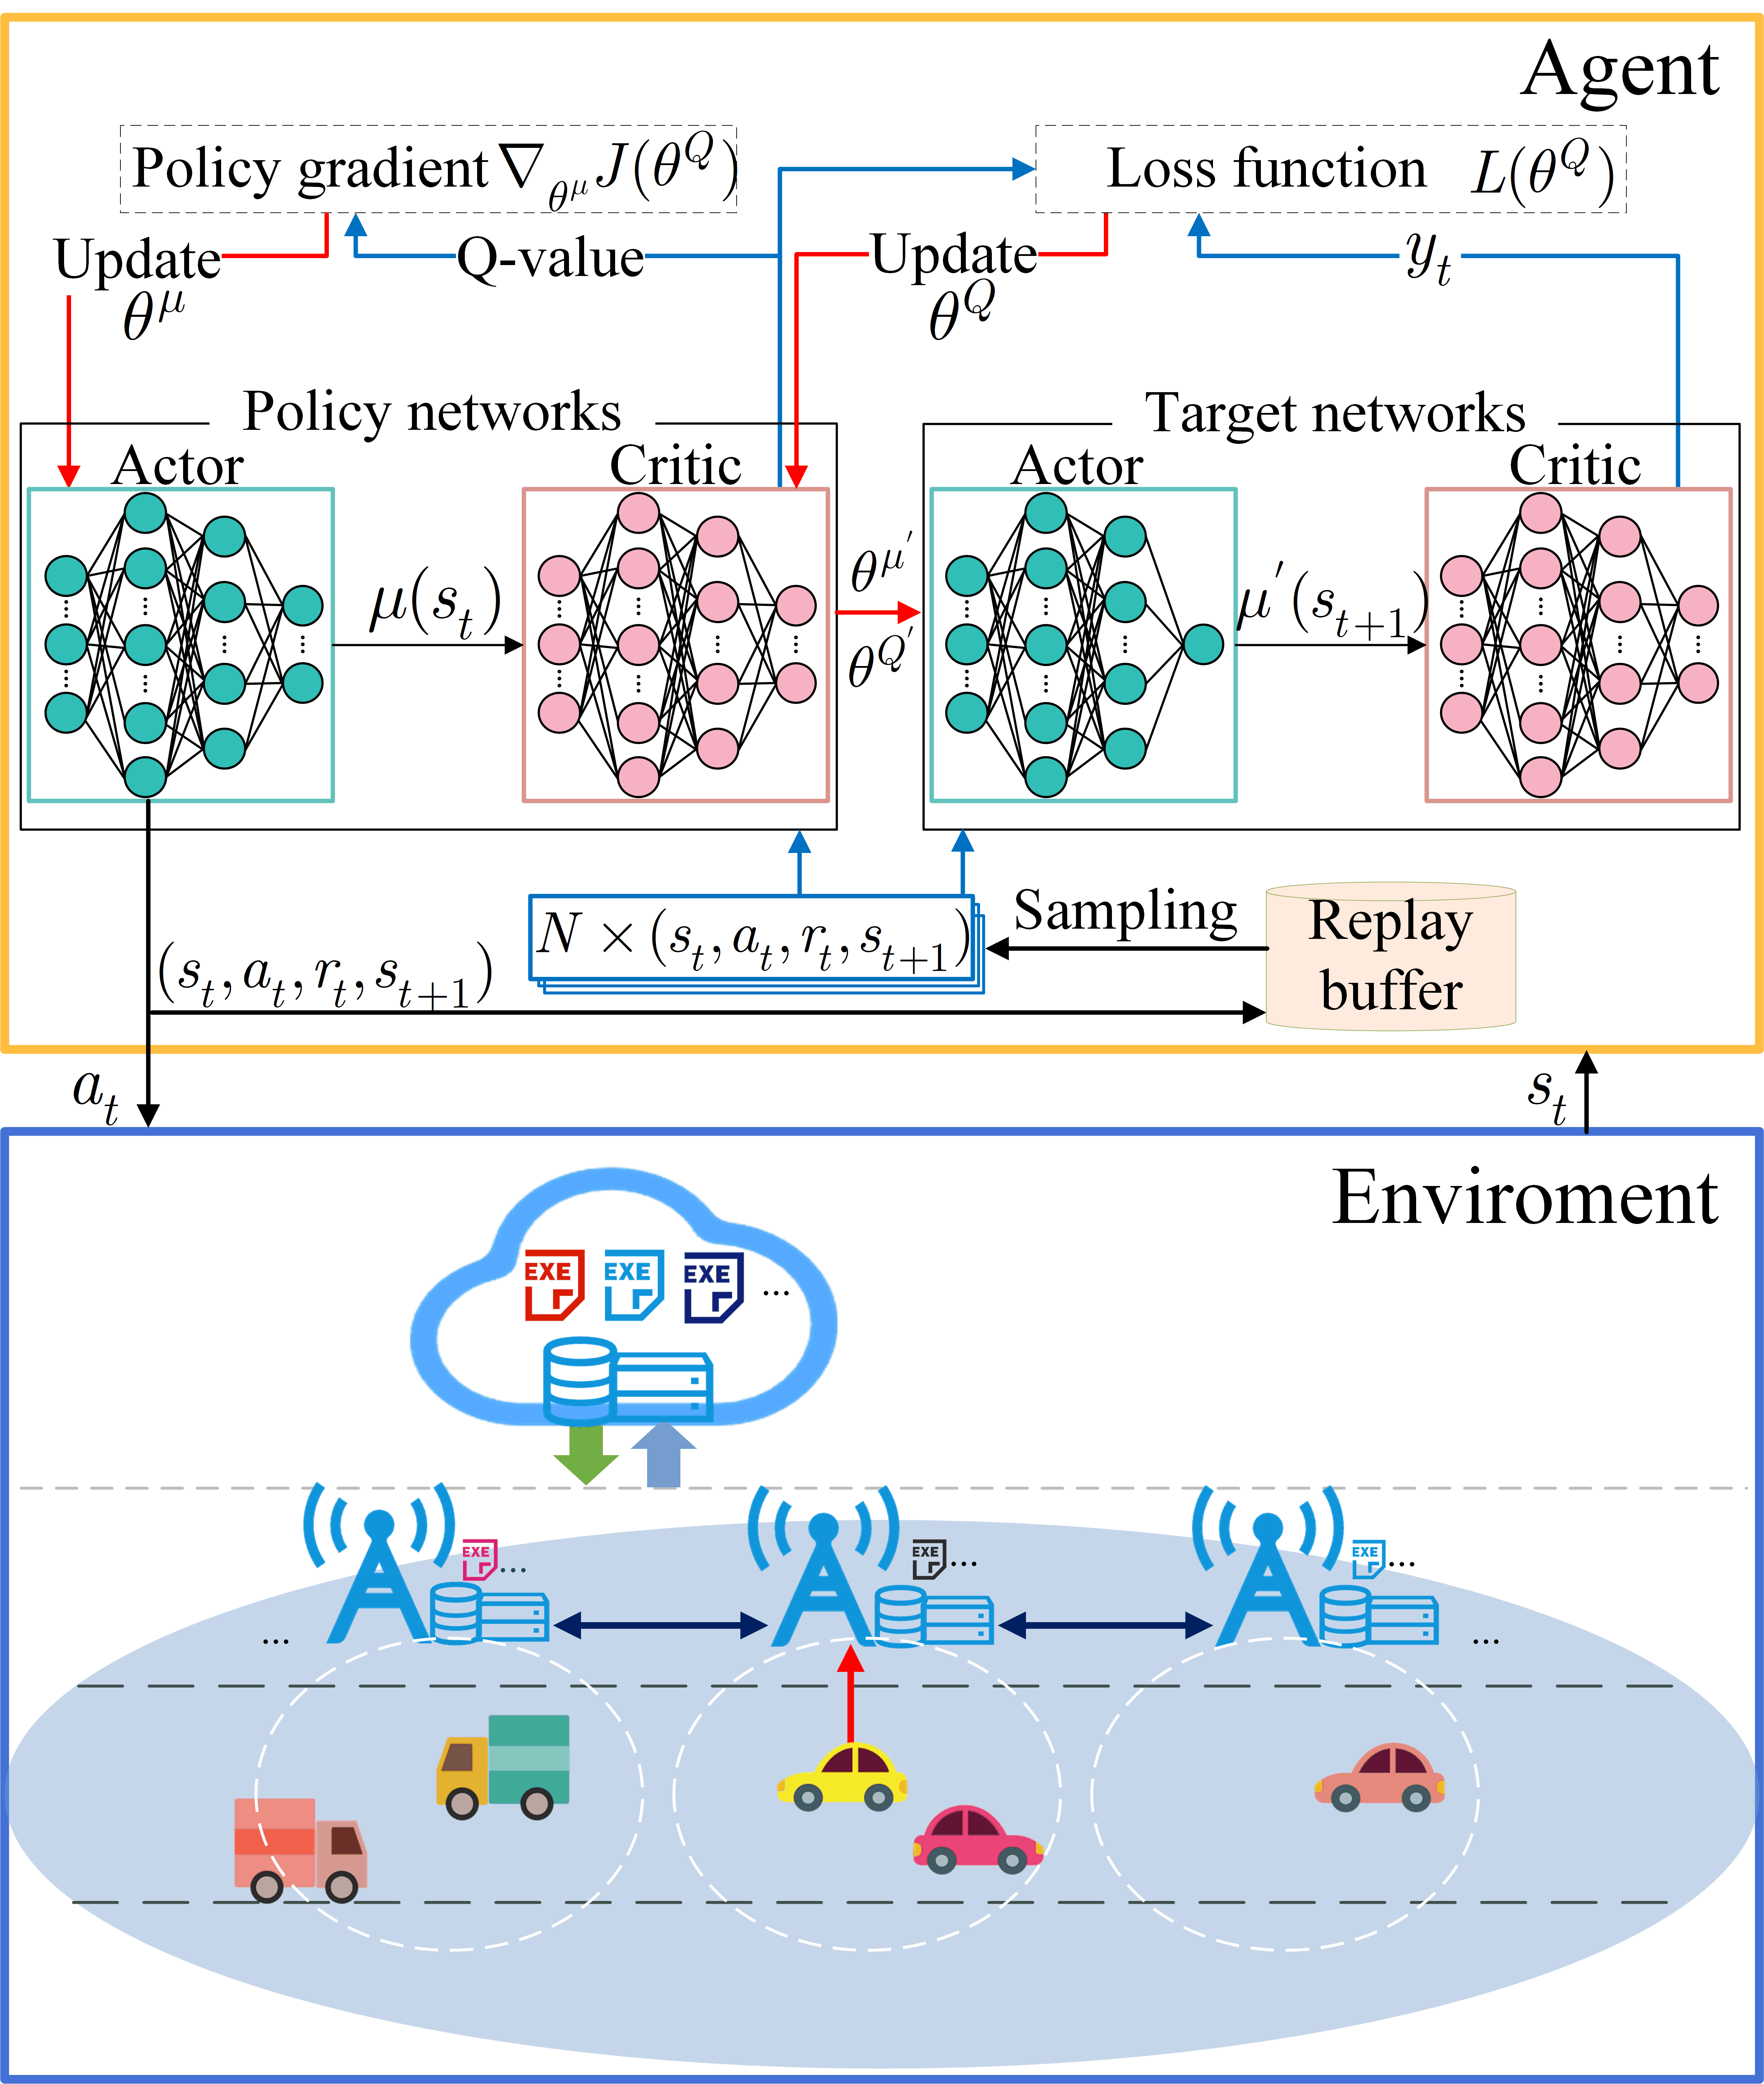
\includegraphics[width=3in]{DRLSCCO.png}
	\caption{The framework of the DRLSCCO.}
	\label{fig: DRLSCCO}
\end{figure}

In the proposed DRLSCCO scheme, a specific state-action pair $ (s_t,a_t) $ is sampled from $ \mathbf{S}(t) \times \mathbf{A}(t) $, where $ s_t\in \mathbf{S}(t) $, $ a_t\in \mathbf{A}(t) $.
As shown in Fig. \ref{fig: DRLSCCO}, the policy actor network implement the deterministic policy function $\mu(s_t|\theta^{\mu})$, which maps the current state $ s_t $ to a deterministic action $ a_t $, i.e., $ a_t = \mu(s_t|\theta^{\mu}) $. The policy critic network estimate the  Q-value (i.e., action-value function) $Q(s_t, a_t|\theta^{Q})$, obtained by taking action $ a_t $ in state $ s_t $, which  represents the expected cumulative discounted reward and can be expressed as
\begin{equation}
	\label{equ: Q-value}
	Q(s_t, \mu(s_t|\theta^{\mu})|\theta^{Q}) = \mathbb{E}_{s_{t+1}\sim \mathrm{P}} \left[ \sum_{k=0}^{\infty}{\alpha^{k}r_{t+k}} \right].
\end{equation}
Equation \eqref{equ: Q-value} satisfies a recursive relationship called Bellman equation, which can be written as
\begin{equation}
	\label{equ: Bellman}
	\begin{aligned}
		Q(s_t, \mu(s_t|\theta^{\mu})|\theta^{Q}) = &  \mathbb{E}_{s_{t+1}\sim \mathrm{P}} \big[  \alpha Q(s_{t+1}, \mu(s_{t+1}|\theta^{\mu})|\theta^{Q})  \\ 
												  & + r_t  \big].
	\end{aligned}
\end{equation}
Here, $ \alpha $ is the discount factor; $ \theta^{\mu} $ and $ \theta^{Q} $ denote the parameters of the actor and critic networks in the policy networks, respectively. 
Although the state transition probability is not explicitly modeled in this problem, the transition is implicitly defined and implemented by the simulation environment. Therefore, the expectation $ \mathbb{E}_{s_{t+1} \sim \mathrm{P}} $ is still used in the theoretical formulation to preserve the mathematical completeness and standard representation of the Bellman equation.
To ensure stable training, the target Q-value  $ y_t $ is constructed by replacing the Q-value  and policy with their target networks' counterparts. It is defined as
\begin{equation}
	\label{equ: target Q-value}
	y_t = r_t + \alpha Q^{\prime}(s_{t+1}, \mu(s_{t+1}|\theta^{\mu^{\prime}})|\theta^{{Q^{\prime}}}).
\end{equation}
The target networks are maintained with parameters $ \theta^{\mu^{\prime}}$ and $ \theta^{Q^\prime} $, which are soft updated by slowly tracking the policy networks.

Since DDPG adopts a deterministic policy, the agent may become trapped in local optima during early training due to insufficient exploration. To encourage exploration, a noise term \( n_t \) is added to the action, yielding the modified action $ a_t $.
\begin{equation}
	\label{equ: obtain action}
	a_t = \mu(s_t|\theta^{\mu}) + n_t.
\end{equation}
To reduce the correlation between consecutive experiences, DDPG employs a replay buffer to store interaction tuples of the form $ (s_t, a_t, r_t, s_{t+1})  $.
At each time slot, after the agent selects an action $ a_t $ and receives the corresponding reward $ r_t $ and next state $ r_{t+1} $, the transition $ (s_t, a_t, r_t, s_{t+1})  $ is stored in the experience replay buffer. 
The  data randomly sampled from the replay buffer is  used for updating the parameters of the policy networks.

Now that experience replay buffer provides samples of mini-batch of transitions, 
the critic network $ \theta^{Q} $ is updated by minimizing the mean squared error (MSE) between the  Q-value and the target Q-value. The loss function is defined as
\begin{equation}
	\label{equ: loss function for update critic sitaQ}
	L(\theta^{Q}) = \frac{1}{N}\sum_{i=1}^{N}\left( y_i - Q \left( s_i, \mu\left( s_i|\theta^{\mu} \right)|\theta^{Q} \right) \right)^2,
\end{equation}
where $ N $ is the mini-batch size sampled from the experience replay buffer.
The actor network parameter $ \theta^{\mu}$ is updated using the sampled deterministic  policy gradient, which aims to maximize the Q-value and can be expressed as
\begin{equation}
	\label{equ: policy gradient ascent for update actor sitamu}
	\begin{aligned}
		\nabla_{\theta^{\mu}} J(\theta^{Q})= & \frac{1}{N}\sum_{i=1}^{N}\left[ \nabla_{a}Q\left( s,a|\theta^{Q} \right)|_{s=s_i,a=\mu(s_i|\theta^{\mu})} 	\right.		\\
		& \left. \cdot \nabla_{\theta^{\mu}}\mu (s|\theta^{\mu})|_{s=s_i} \right].
	\end{aligned}
\end{equation}
Therefore, the critic and actor parameters are updated by gradient descent and gradient ascent, which as follows:  
\begin{equation}
	\theta^{Q} \leftarrow \theta^{Q} - \eta \cdot \nabla_{\theta^{Q}}(L(\theta^{Q}))
\end{equation}
and
\begin{equation}
	\theta^{\mu} \leftarrow \theta^{\mu} + \eta \cdot \nabla_{\theta^{\mu}}(J(\theta^{\mu})),
\end{equation}
where $ \eta $ denote learning rate.
The target networks are not directly copied from the policy networks but updated using a soft update mechanism, which slowly tracks the policy networks' parameters. At each iteration, the target networks' parameters $ \theta^{\mu^{\prime}} $ and $ \theta^{Q^{\prime}} $ are updated according to
\begin{equation}
	\label{equ: target1}
	\theta^{Q^{\prime}} \leftarrow \tau \theta^{Q} + (1-\tau)\theta^{Q^{\prime}}
\end{equation}
and
\begin{equation}
	\label{equ: target2}
	\theta^{\mu^{\prime}} \leftarrow \tau \theta^{\mu} + (1-\tau)\theta^{\mu^{\prime}}.
\end{equation}
Here, $ 0 < \tau \ll 1 $ is a smoothing factor, which prevent excessive fluctuations in the target Q-value during learning.  
Through the above process, the agent gradually optimizes decision-making strategy, enabling it to efficiently perform service caching and   offloading  decisions in complex VEC environment. The complete DRLSCCO scheme is detailed in Algorithm \ref{alg: DRLSCCO}.

\begin{algorithm}
	\caption{The DRLSCCO Scheme for Service Caching and Computation Offloading.}
	\label{alg: DRLSCCO}
	\renewcommand{\algorithmicrequire}{\textbf{ Input:}}
	\renewcommand{\algorithmicensure}{\textbf{ Output:}}
		\begin{algorithmic}[1]
		\REQUIRE  
		$ \mathcal{N} $, $ \mathcal{L} $, $ \mathcal{T} $, $ \mathcal{K} $, $ \mathcal{J}_{t} $, $ \mathcal{K}_{j} $, $ \mathcal{C}_{n} $.
		\ENSURE   
		The optimal policy actor network parameter $ \theta^{\mu} $.
		\STATE 
		Initialize networks :
		the policy actor network parameter $ \theta^{\mu} $;  
		the policy critic network parameter $ \theta^{Q} $; 
		the target actor network parameter $ \theta^{\mu^{\prime}} $;
		the target critic network parameter $ \theta^{Q^{\prime}} $;
		the soft update coefficient $ \tau $;
		the number of episodes $ I $;
		the batch sample size $ e $; 
		the replay buffer size $ E $;
		the random noise $ n_{t} $.
		\STATE Initialize empty experience replay buffer.
		\FOR {$ i=1, 2, \dots, I $}
			\STATE Initialize the observation state $ s_0 $ of  time slot $ 0 $ with the input.
			\FOR {$ t=0,1, \dots, T-1 $}
				\STATE The agent selects an action $ a_t $  according to \eqref{equ: obtain action}.
				\STATE Vehicles and edge servers execute the selected action $ a_t $.
				\STATE The agent observes the next state $ s_{t+1} $ and receives an immediate reward $ r_t $.
				\STATE Store transition $ (s_t, a_t, r_t, s_{t+1}) $ in experience replay buffer.
				\IF {the replay buffer size exceeds a predefined threshold}
					\STATE Randomly sample a mini-batch of $ e $ transitions $ (s,a,r,s_{\text{next}}) $ from the replay buffer.
					\STATE Calculate the Q-value by \eqref{equ: Q-value}.
					\STATE Calculate the target Q-value $ y $ by \eqref{equ: target Q-value}.
					\STATE Update the critic network parameter $ \theta^{Q} $ by minimizing the loss function  defined in \eqref{equ: loss function for update critic sitaQ}.
					\STATE Update the actor network parameter $ \theta^{\mu} $  \eqref{equ: policy gradient ascent for update actor sitamu}.
					\STATE Perform a soft update on the target networks' parameters $ \theta^{Q^{\prime}} $ and $ \theta^{\mu^{\prime}} $ according to \eqref{equ: target1} and \eqref{equ: target2}, respectively.
				\ENDIF
			\ENDFOR
		\ENDFOR
		\end{algorithmic}
\end{algorithm}


% /algorithm2e格式
% \begin{algorithm}[H]
%     \SetAlgoLined
%     \KwIn{
%         $ \mathcal{N} $, $ \mathcal{L} $, $ \mathcal{T} $, $ \mathcal{K} $, $ \mathcal{J}_{t} $, $ \mathbf{f}_{j}(t) $, $ \mathcal{K}_{j} $, $ \mathcal{C}_{n} $, $ \mathbf{S}(0) $
%     }
%     \KwOut{the optimal policy actor network parameter $ \theta^{\mu} $}
%     initialize networks: the policy actor network parameter $ \theta^{\mu} $;  
%     the policy critic network parameter $ \theta^{Q} $; 
%     the target actor network parameter $ \theta^{\mu^{\prime}} $;
%     the target critic network parameter $ \theta^{Q^{\prime}} $;
%     the soft update coefficient $ \tau $;
%     the number of episodes $ I $; 
%     the batch sample size $ e $; 
%     the replay buffer size $ E $;
%     the random noise $ n_{t} $\;
%     initialize empty experience replay buffer\;
%     \For{$ episode =1,2, \dots, I $}{
%         initialize the observation state $ s_0 $ of  time slot $ 0 $ with input
% 		parameters\;
%         \For{$ t=0,1, \dots, T-1 $}{
%             the agent selects an action $ a_t $  according to \;
%             vehicles and edge servers execute the selected action $ a_t $\;
%             the agent observes the next state $ s_{t+1} $ and receives an immediate reward $ r_t $\;
%             store transition $ (s_t, a_t, r_t, s_{t+1}) $ in experience replay buffer\;
%             \If{the replay buffer size exceeds a predefined threshold}{
%                 randomly sample a mini-batch of $ e $ transitions $ (s,a,r,s_{next}) $ from the replay buffer\;
%                 calculate the Q-value by \;
%                 calculate the target Q-value $ y $ by \;
% 				update the critic network parameter $ \theta^{Q} $ by minimizing the loss function  defined in \;
% 				update the actor network parameter $ \theta^{\mu} $ by \;
% 				perform a soft update on the target networks' parameters $ \theta^{Q^{\prime}} $ and $ \theta^{\mu^{\prime}} $ according to, respectively\;
%             }
%         }
%     }  
%   \caption{The DRLSCCO Scheme for Service Caching and Computation Offloading}
%   \label{alg: DRLSCCO}
% \end{algorithm}

\section{Simulation Experiments and Performance Analysis}
In this section, we analyze the performance of the proposed DRLSCCO scheme by conducting simulation experiments under different parameter settings to emulate various scenarios. 
We use Python 3.8 and PyTorch 2.1.2 to simulate the proposed system model in our study and implement the DRLSCCO scheme.
The simulation environment considers a three-layer VEC system, consisting of a cloud server, edge nodes and vehicles. 
The primary parameters used in the experiments are summarized in Table \ref{tab: experiment parameters}, with some parameter settings referenced from previous studies \cite{SB, GZ}. 
\begin{table}
	\caption{Parameter Setting}
	\label{tab: experiment parameters}
	\begin{center}
		% \renewcommand\arraystretch{1.2}
		\begin{tabularx}{\linewidth}{X p{4.7cm} X}
		\hline
		\textbf{Parameter} 	& \textbf{Meaning} & \textbf{Value}  							\\ \hline
			$ lr_a $		&	The learning rate of actor network			&	$ 0.001 $	\\
			$ lr_c $		&	The learning rate of critic network			&	$ 0.002 $	\\
			% $ \tau $		&	The soft update coefficient					&	$ 0.001 $	\\ 
			$ \gamma $		&	The discount factor							&	$ 0.99 $	\\
			$ e $			&	The sample batch size						&	$ 256 $		\\
			% $ E $			&	The size of replay buffer					&	$ 10000 $	\\
			% $ \Delta t $	& The duration of each time slot  				&  $ 30 $ s		\\
			$ \rho^{max} $ & The max density of vehicles within range of each edge node & $ 10 $																				\\
			$ N $			& The number of edge nodes 						& $ 3 $ 																			  \\
			$ K $			& The number of service types					& $ 3 $ 																			\\
			$ \beta $		& The data size of each service					& $ 30 $ Mb 		\\
			$ d_j(t) $			& The data size of each task					& $ 20 $ Mb	\\
			% $ \lambda $		& The computation density				& $10^5$ 			\\
			% $ f^{V} $			& The CPU frequency of each vehicle				& $ 3 \times 10^8 $ \\
			% $ f^{R} $			& The CPU frequency of each edge server			& $ 6 \times 10^8 $ \\
			$ S^{V} $			& The storage capacity of each vehicle			&$ 30 $ Mb 			\\
			$ S^{R} $			& The storage capacity of each edge server		&$ 50 $ Mb 			\\
		$ r^{e2e} $			& The transmission rate between edge nodes				&$ 10 $ Mbps \\
		$ r^{e2c} $			& The transmission rate from edge node to cloud server	&$ 8 $  Mbps \\
		$ p^{edge} $			& The transmission power  between edge nodes			&$ 1 $ W 	\\
		$ p^{e2c} $			& The transmission rate from edge node to cloud server  &$ 2$  W 	\\
		\hline
		\end{tabularx}
	\end{center}
\end{table}


To comprehensively evaluate the proposed DRLSCCO scheme, we compare it with four service caching and computation offloading benchmark methods:
\begin{enumerate}
	\item 
	No comparative edge nodes (NCE): Subtasks are restricted to three execution options: local execution, (partial) offloading to directly connected edge nodes, or offloading to the cloud server. The cooperative interactions between edge nodes are disabled.
	\item
	LRU-based service caching on vehicles and edge nodes (LRUSC): If the agent attempts to cache a new service, but the cache capacity is insufficient, it replaces the least recently used service.
	\item 
	Random service caching and computation offloading (RSCCO): The caching behavior of vehicles and edge nodes is randomized. Additionally, if a subtask is partially offloaded, its offloading ratio is also determined randomly.
	\item
	No edge nodes (NE): In this case, edge nodes are removed from the system, and subtasks can only be executed locally or offloaded to the cloud server.
\end{enumerate}


\begin{figure}
	\centering
	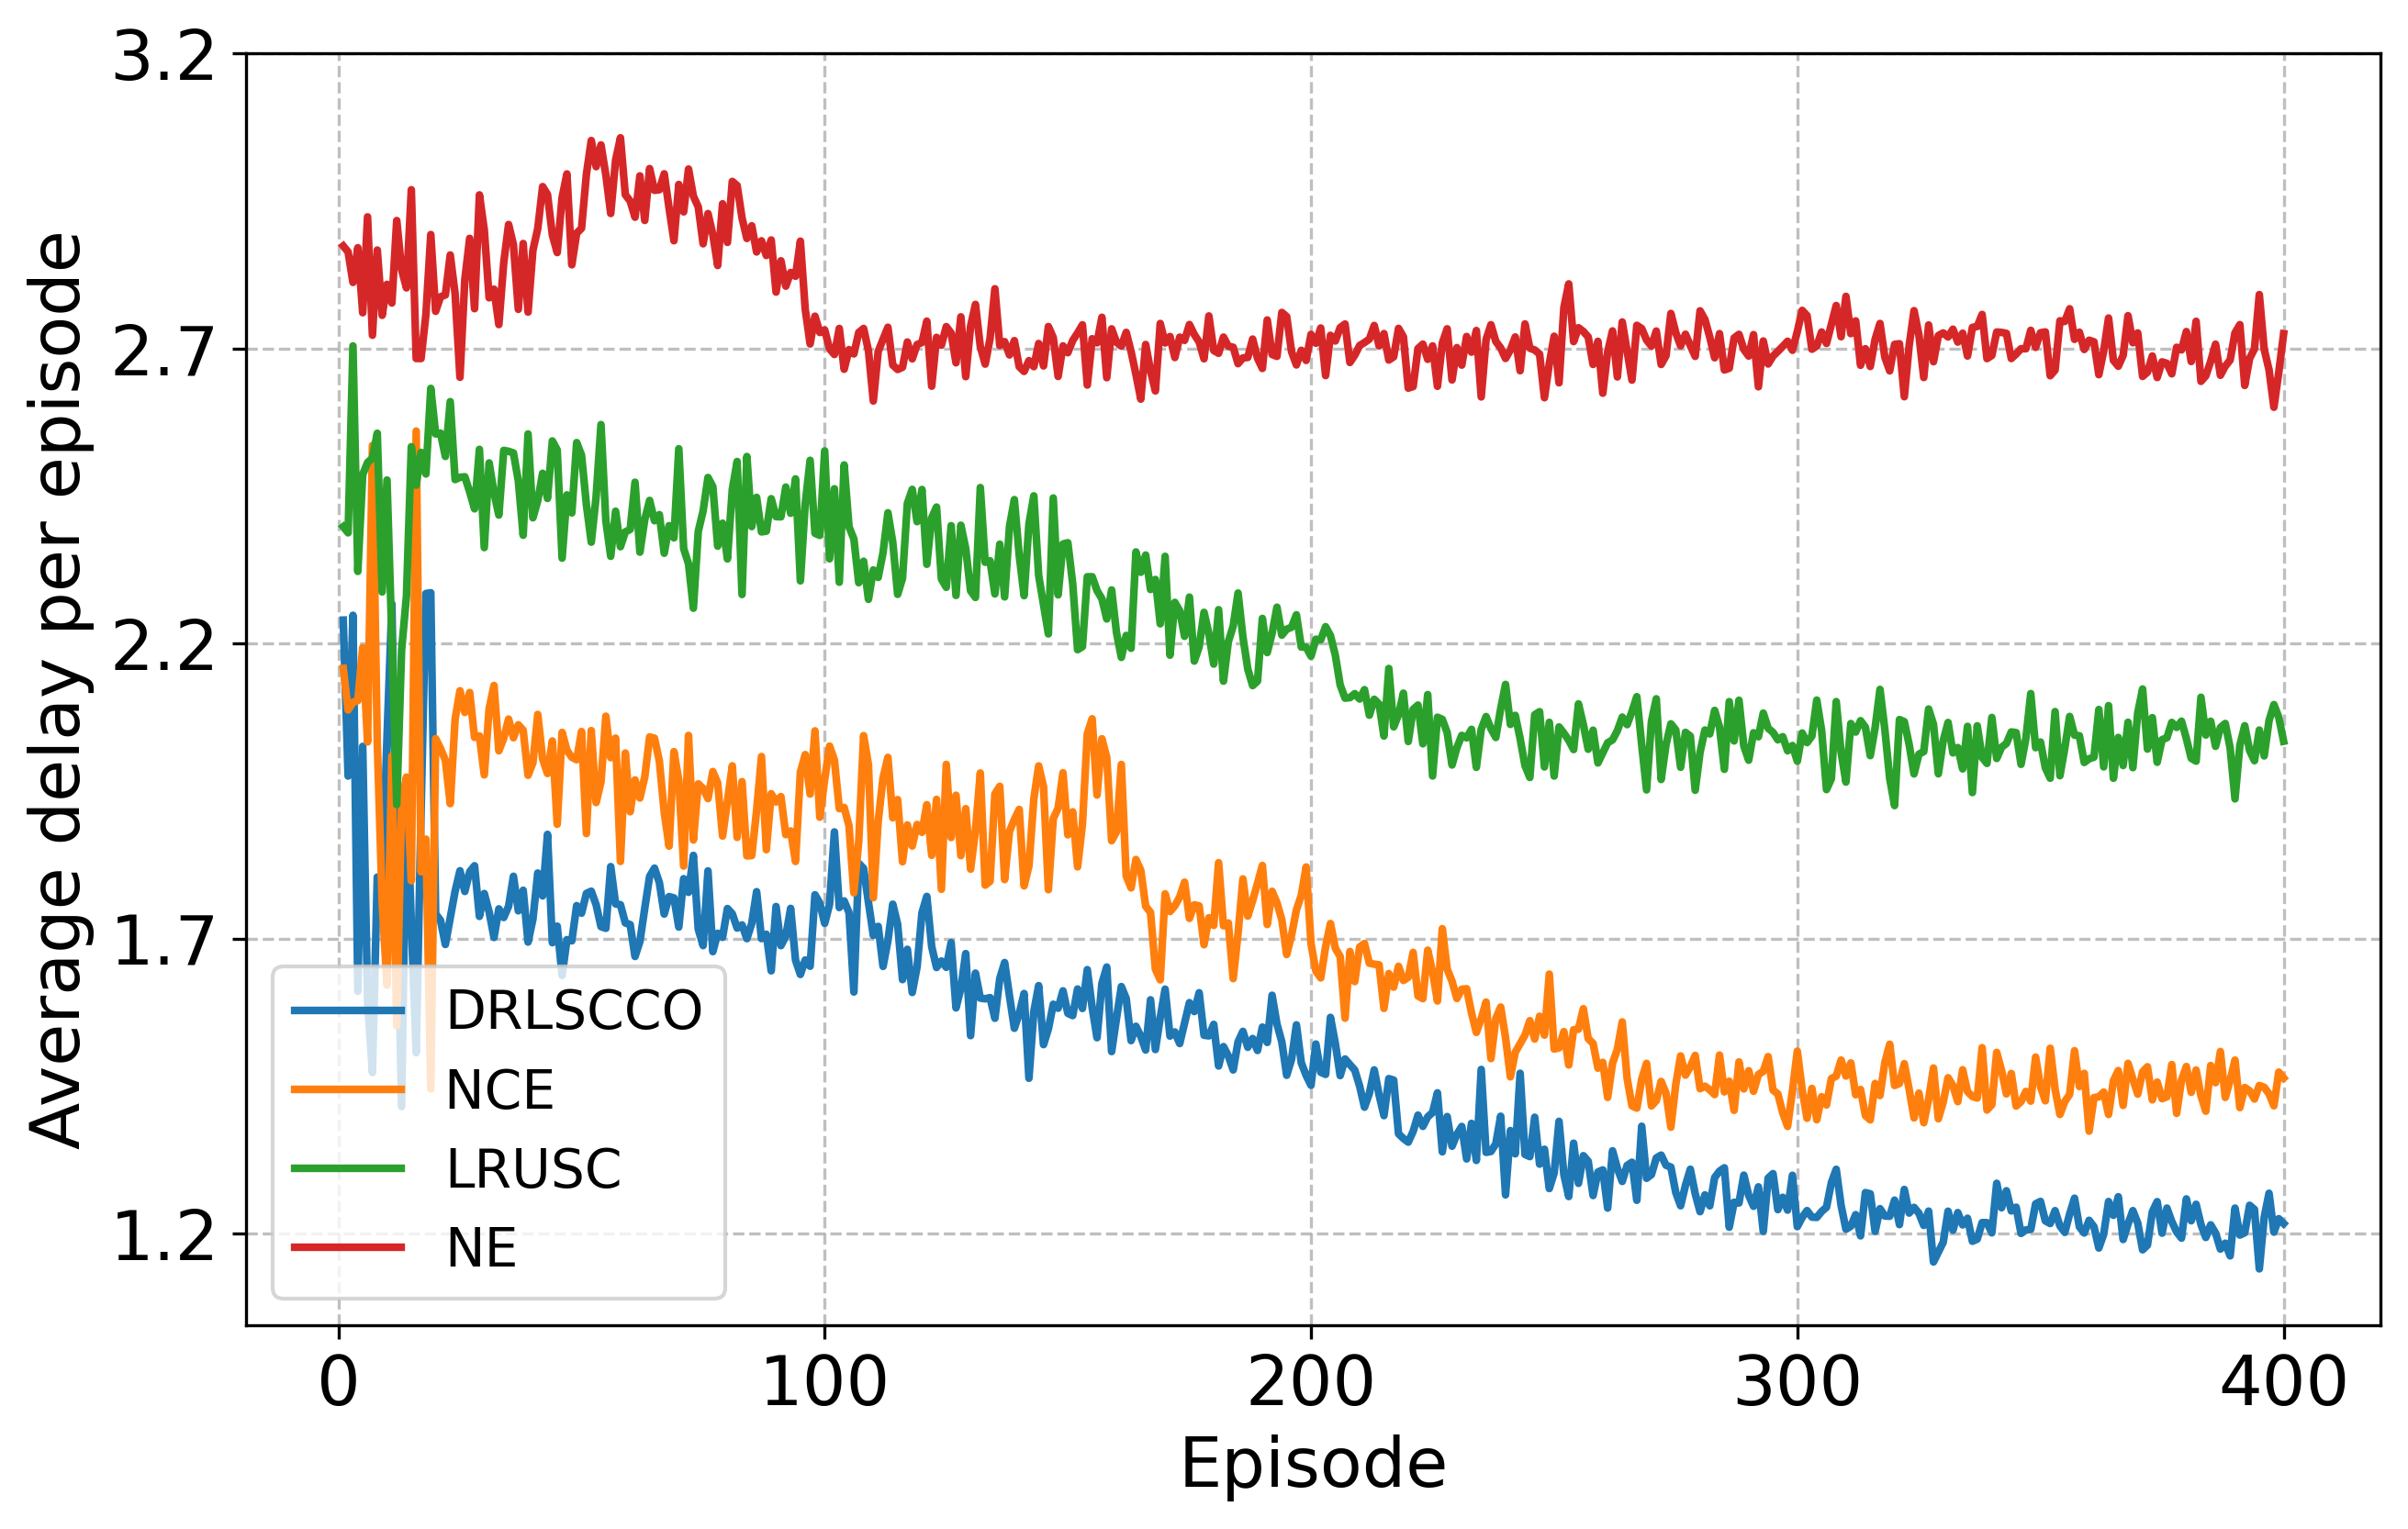
\includegraphics[width=3in]{convergence_delay.png}
	\caption{The performance of average delay per episode}
	\label{fig: convergence 1}
\end{figure}

\begin{figure}
	\centering
	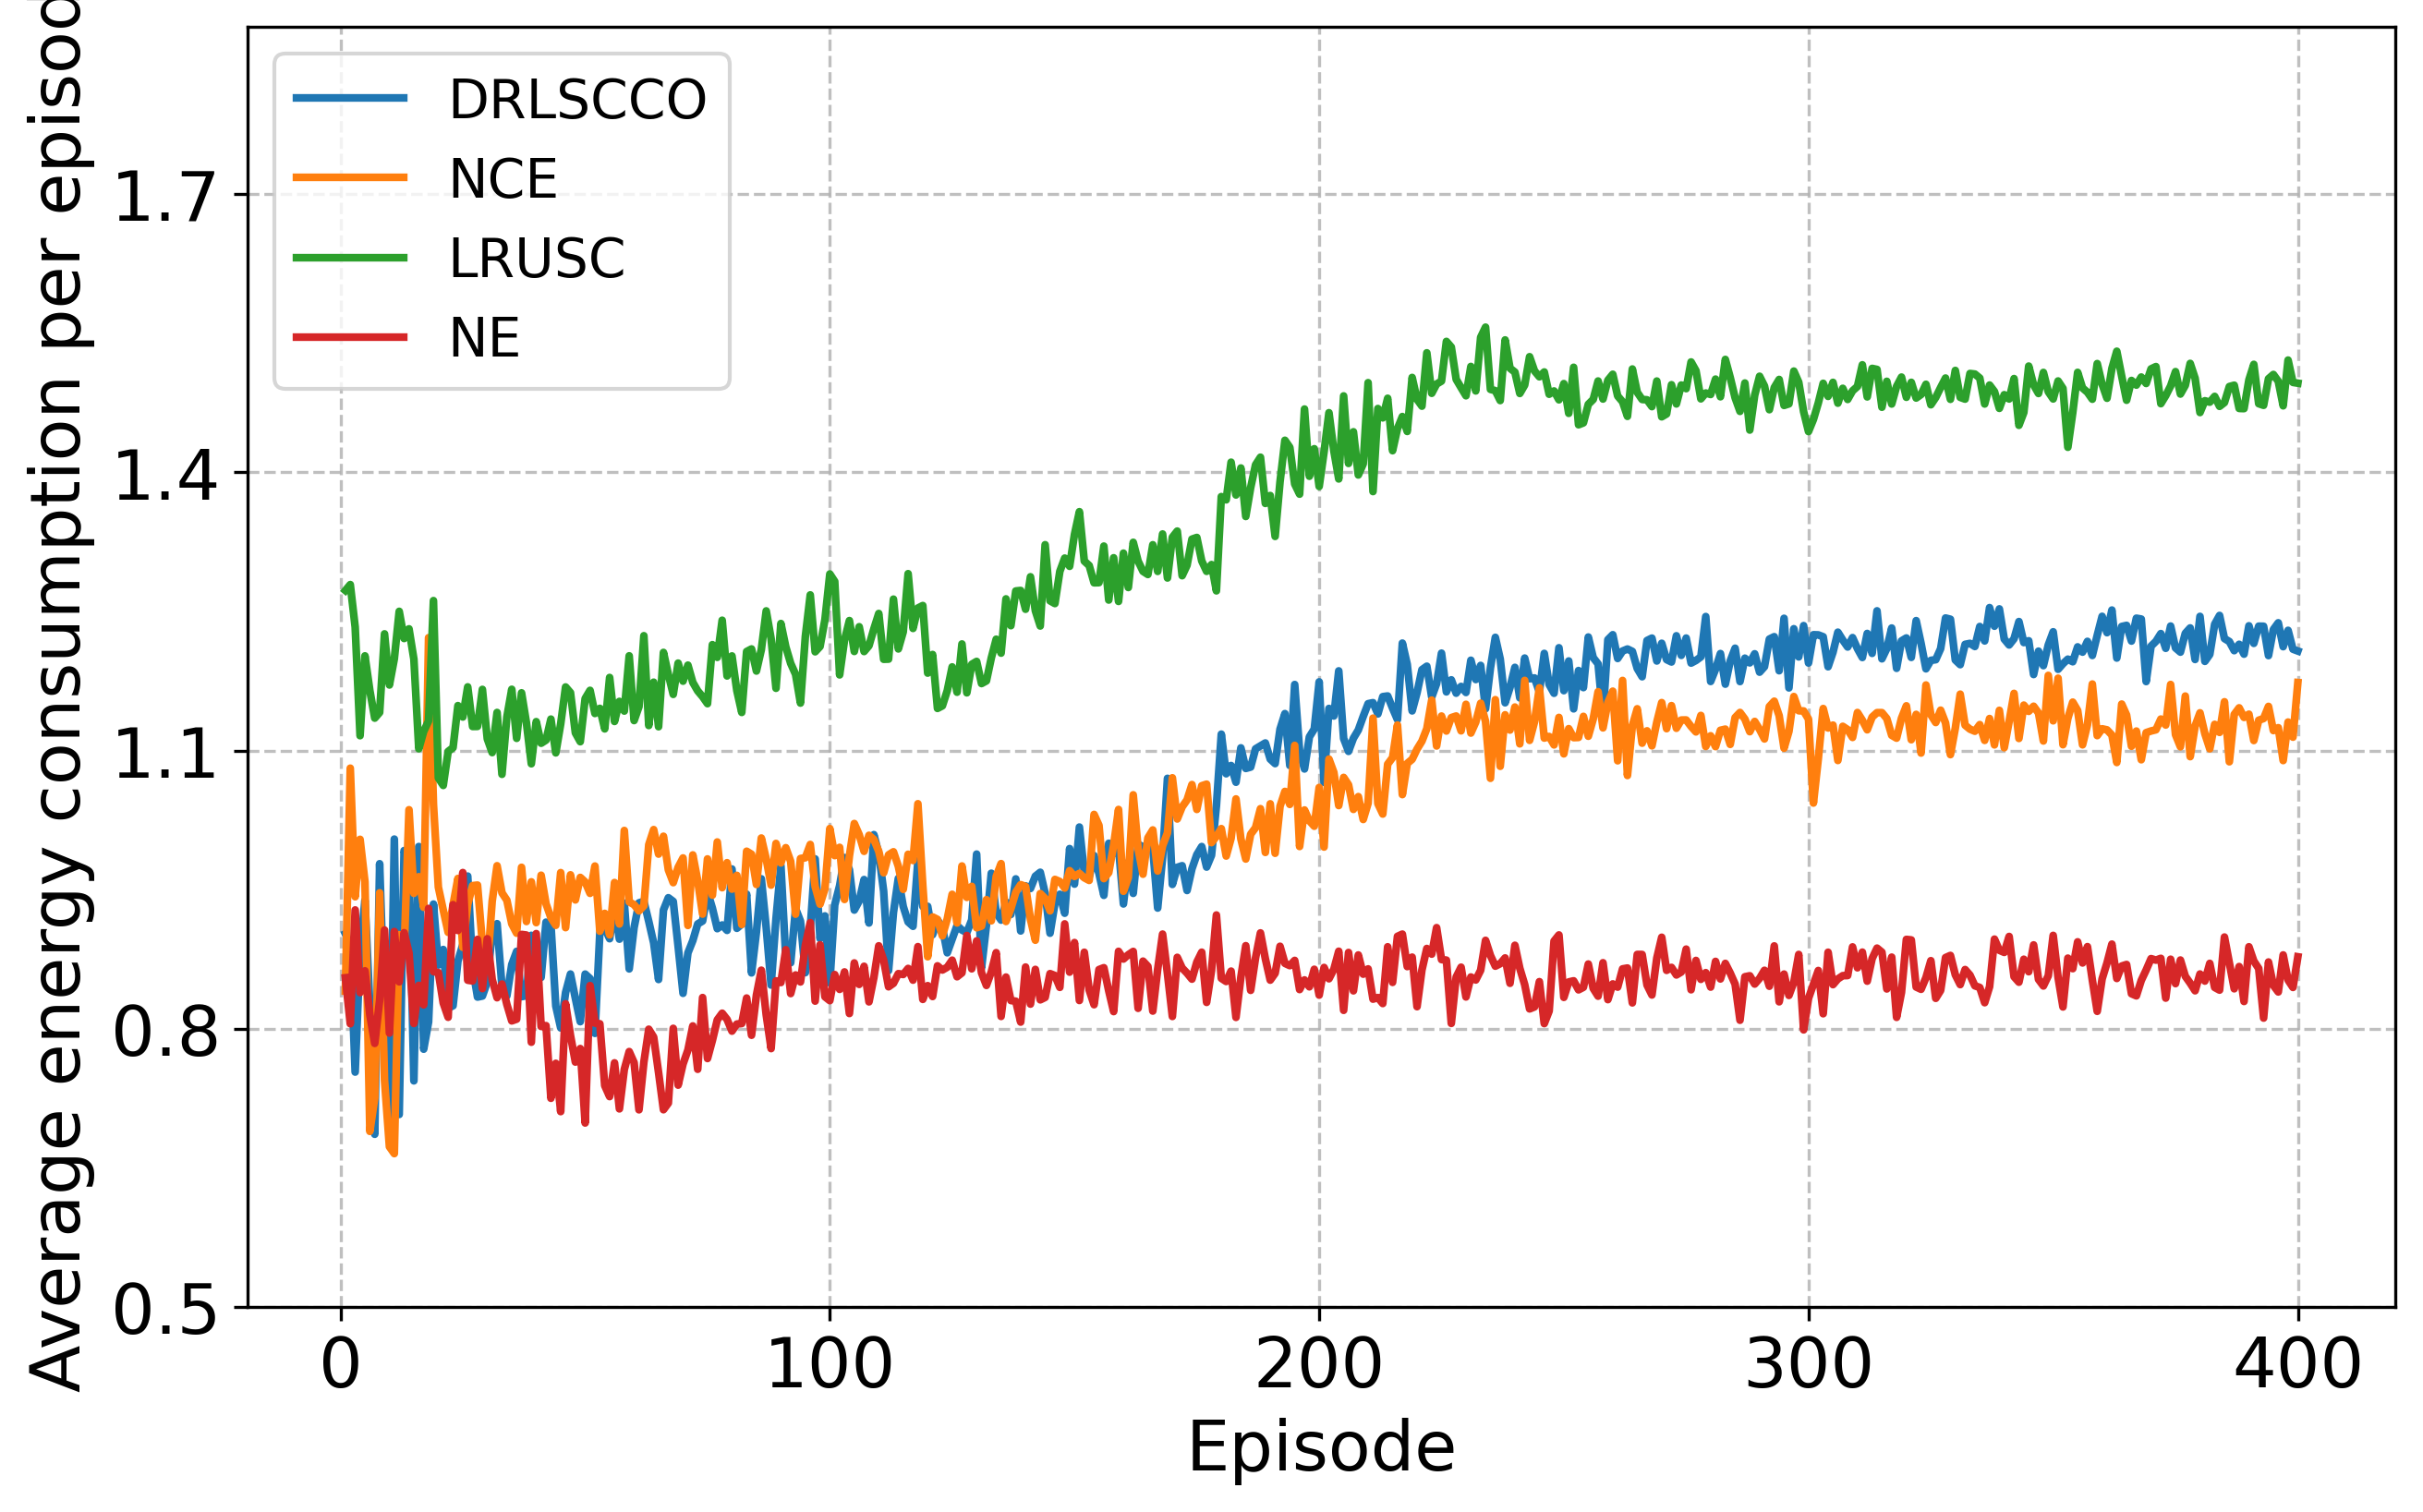
\includegraphics[width=3in]{convergence_energy.png}
	\caption{The performance of average energy consumption per episode}
	\label{fig: convergence 2}
\end{figure}
% 前两张图收敛的条件: 车辆的密度是一个范围而不是固定值, 但是任务大小固定
First, we compare the average task processing delay per training episode for schemes involving network participation in Fig. \ref{fig: convergence 1}.
Since MNOs' energy consumption is closely related to task processing delay, we further compare the average energy consumption per episode as training progresses in Fig. \ref{fig: convergence 2}.  
Among these,  the average delay of  schemes decreases and gradually stabilizes as the number of episodes increases, while their average energy consumption increases and reach a steady state.
This is because the participation of edge servers and cloud servers deployed by the MNOs reduces task execution delay, while simultaneously increasing the MNOs' energy consumption.
Lacking cooperative caching and offloading, the NCE forces subtasks to be offloaded to the cloud when edge nodes are unavailable, increasing average transmission delay.
The LRUSC, relying solely on past access records for cache replacement, operates more greedily than DRLSCCO and NCE, thus impacting offloading decisions and resulting in higher delay.
In the NE, the absence of edge servers means that task execution delay is primarily determined by computation on vehicle and transmission latency. As a result, it exhibits the highest delay, highlighting the advantages of edge computing.
Overall, these results demonstrate that the proposed scheme, DRLSCCO, continuously optimizes both service caching allocation and subtask offloading scheduling, achieving the lowest delay while keeping the increase in energy consumption within a relatively small range.




\begin{figure}
	\centering
	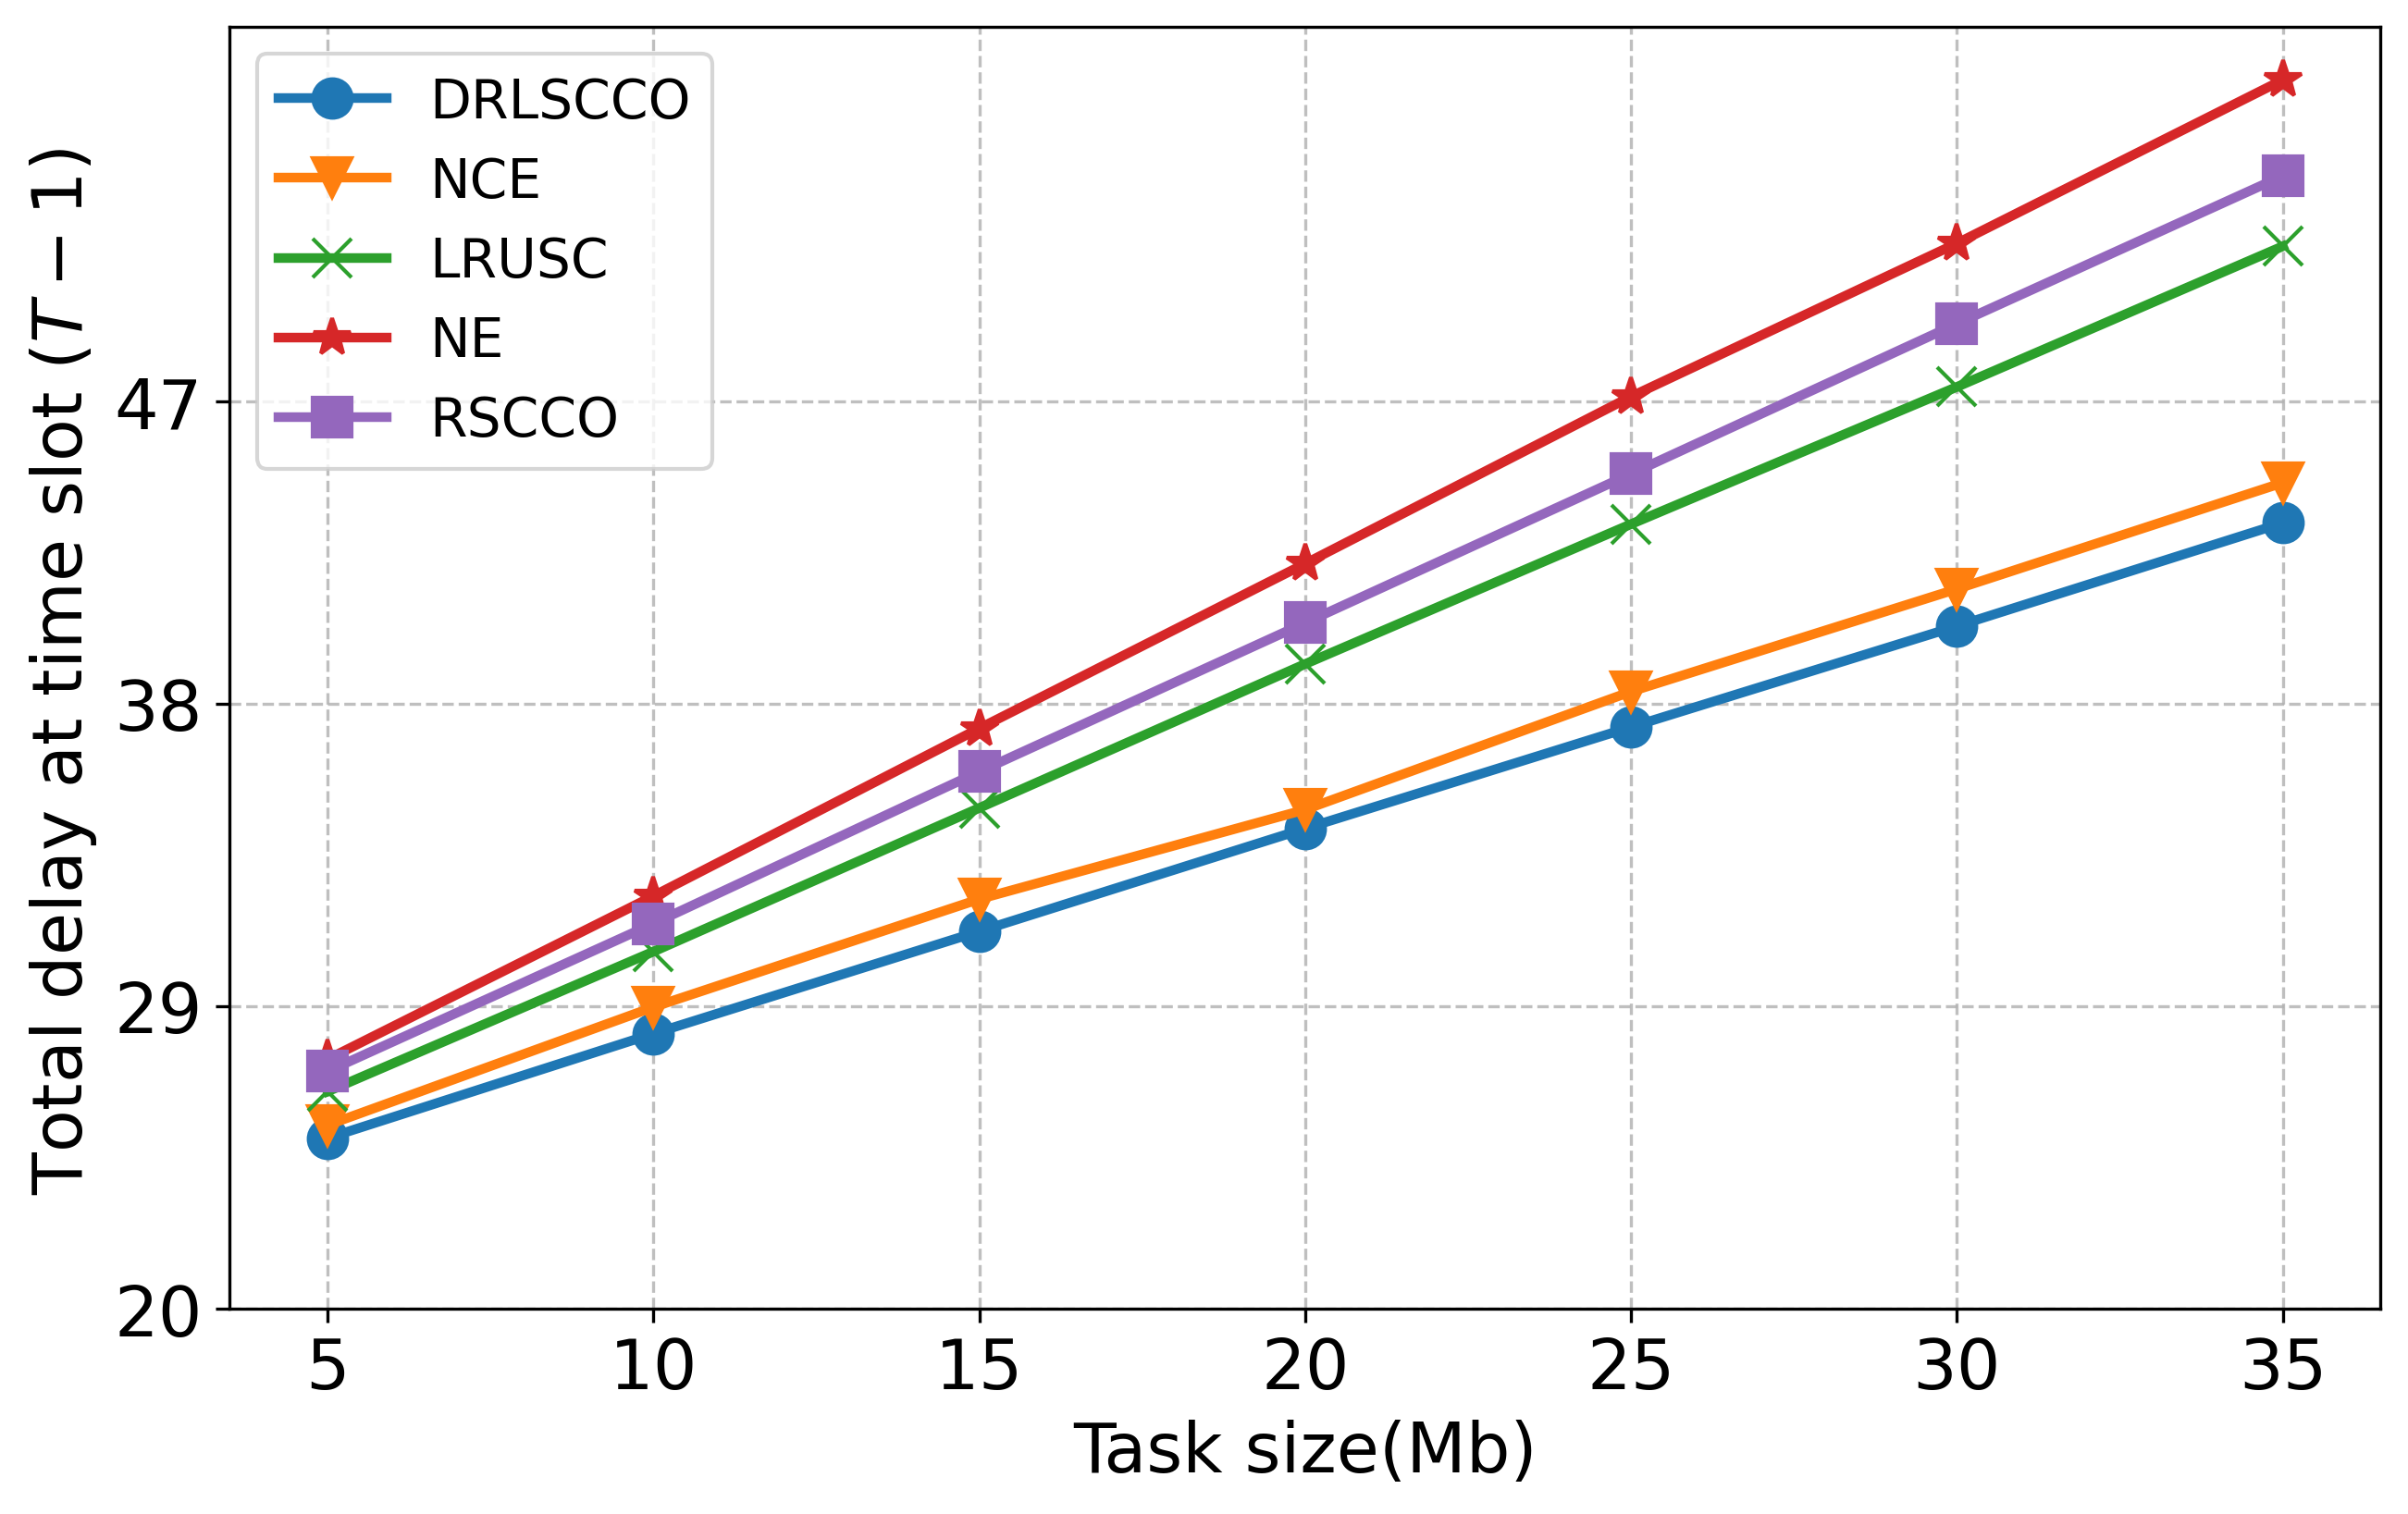
\includegraphics[width=3in]{task_size_delay.png}
	\caption{The influence of task size on delay}
	\label{fig: task size v delay}
\end{figure}
% fig: task_size v delay 该图建立在: 车辆密度固定在最大值, 任务大小区间变化
Then the vehicle density is fixed at $ 10 $ to explore the impact of varying task size on the total delay under all schemes, as shown in Fig.~\ref{fig: task size v delay}. 
% 
As the task size increases from $ 5 $ Mb to $ 35 $ Mb, the total delay increases steadily across all schemes, as expected, due to the positive correlation between delay and subtask size $ d_{j,k}(t) $ in all delay-related formulations.
% 
When the task size is small, the delays of all schemes are relatively close. As the task size increases, the delay differences among the schemes become more pronounced. The NE scheme, which lacks edge servers, exhibits the most significant increase in delay, followed by RSCCO and LRUSC. Compared to DRLSCCO, the NCE scheme offloads more subtasks to the cloud server—corresponding to the service deployment mode M6—thereby resulting in higher delays.
% 
Among all the schemes, the proposed scheme DRLSCCO  consistently achieves the lowest total delay under all task sizes. This demonstrates the effectiveness of the scheme in adapting to varying task loads and optimizing offloading decisions dynamically.



% fig: vehicle density该图建立在: 车辆密度区间, 任务大小固定 
Subsequently, the task size is fixed at $20$ Mb to investigate the impact of vehicle density on task execution delay in Fig.~\ref{fig: vehicle density v delay}.  
The results demonstrate that as vehicle density increases, the average delay of all schemes rises due to increased demand on the communication channel, which reduces per-vehicle bandwidth and leads to higher transmission delays.
When the vehicle density is relatively low, i.e.,  $ \rho^{\max} = 4 $, each vehicle is allocated more bandwidth for task transmission, prompting the agent to offload tasks to the cloud server with higher computing capabilities and thus reducing overall processing delay. Consequently, in low-density scenarios, the NE scheme exhibits a lower average delay compared to LRUSC and RSCCO, both of which involve edge participation, but this advantage vanishes as vehicle density increases.
Notably, the proposed DRLSCCO scheme consistently achieves the lowest task execution delay across varying vehicle densities, highlighting its strong adaptability and effectiveness in dynamic environments.
\begin{figure}[h]
	\centering
	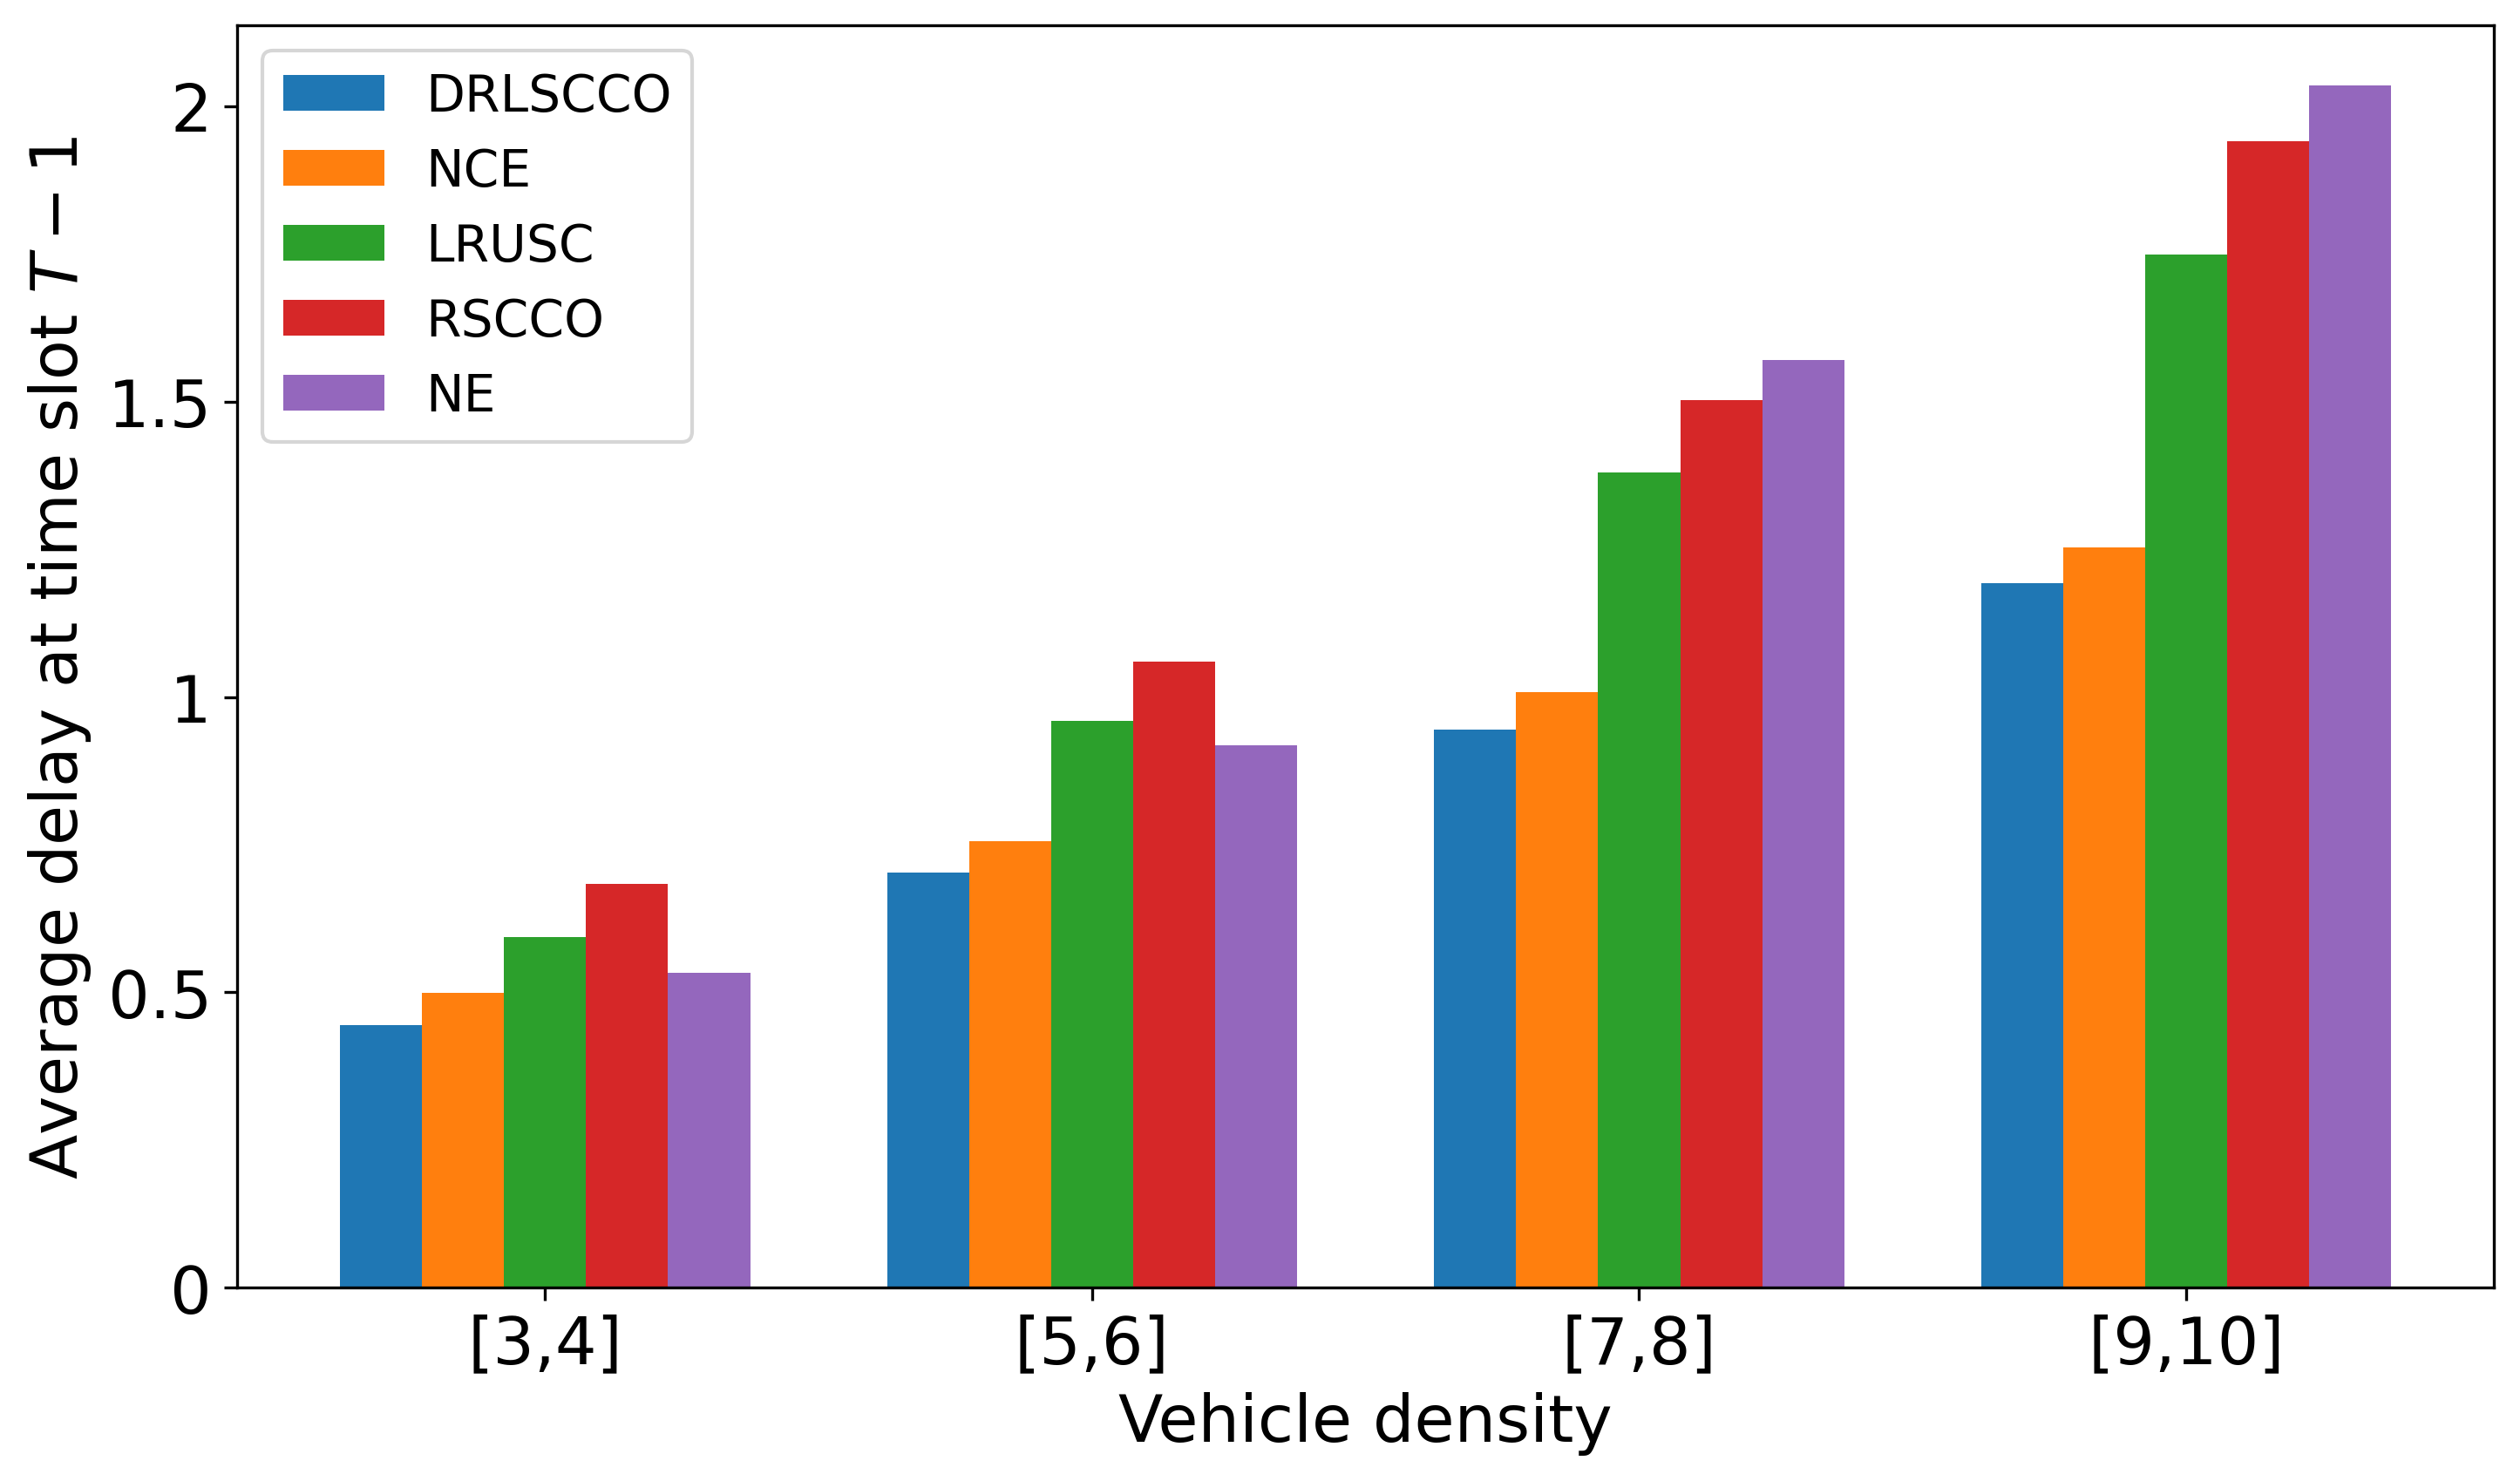
\includegraphics[width=3in]{vehicle_density.png}
	\caption{The influence of vehicle density on delay}
	\label{fig: vehicle density v delay}
\end{figure}


% fig: edge server frequency 
\begin{figure}[h!]
	\centering
	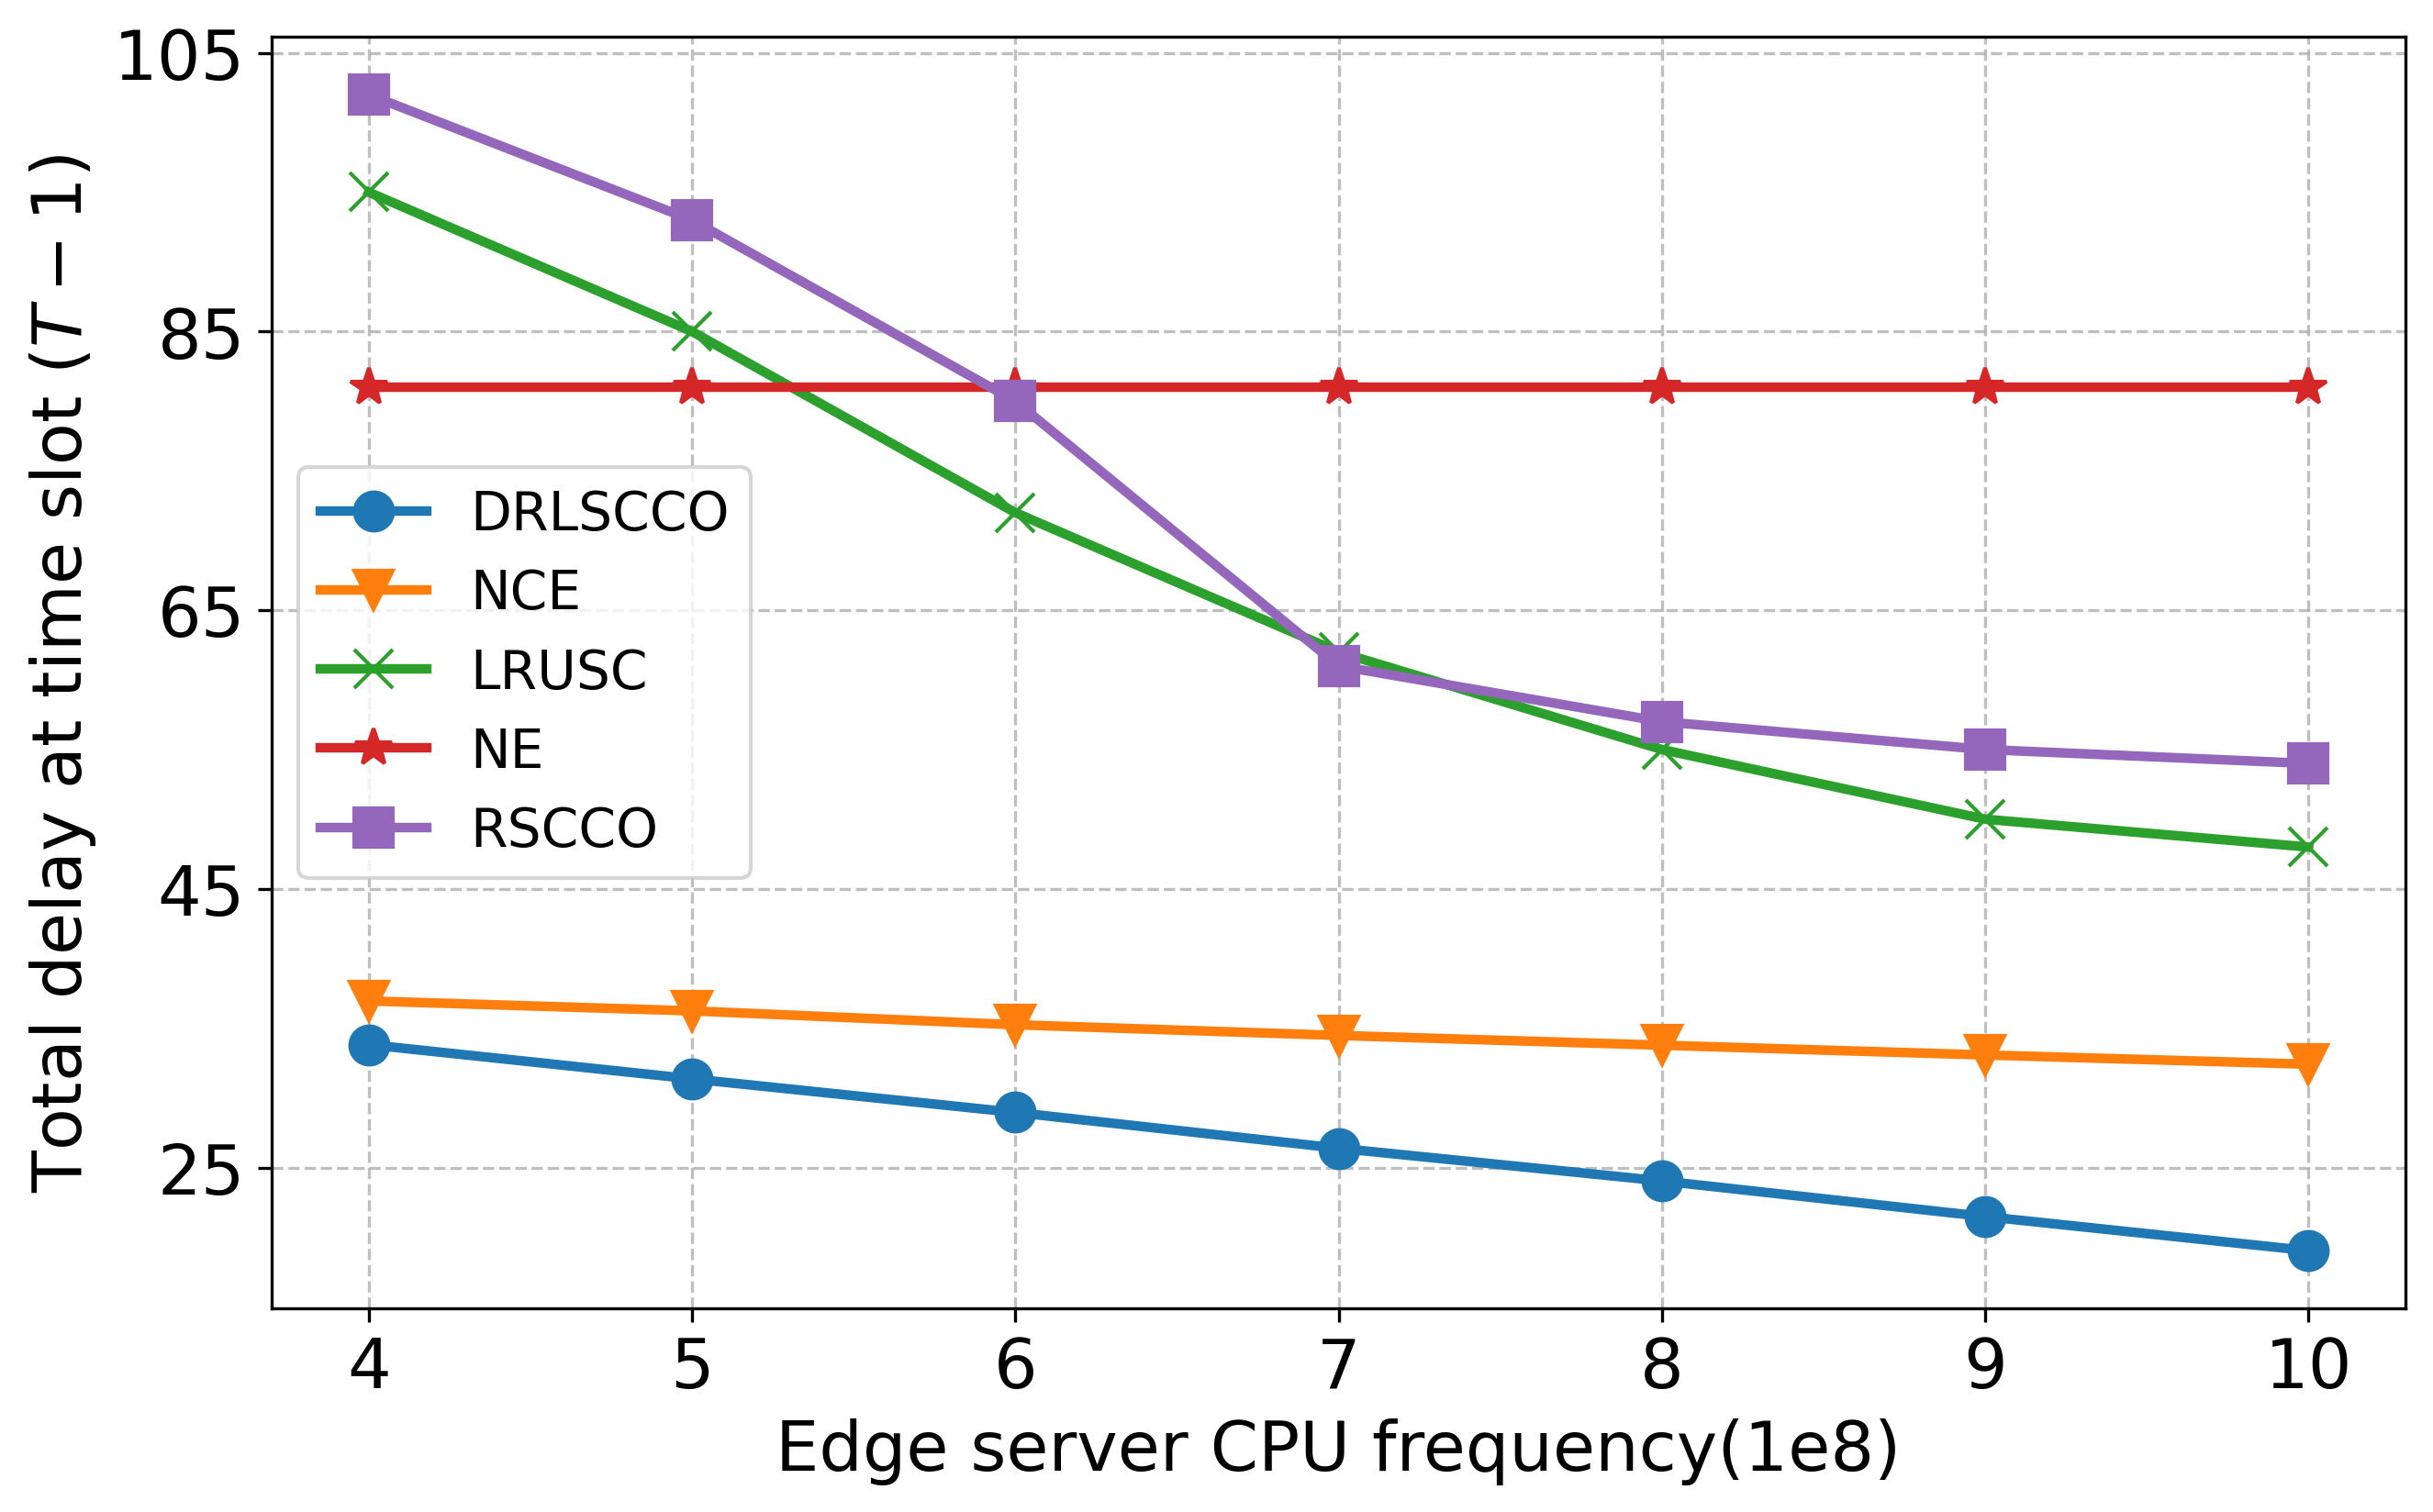
\includegraphics[width=3in]{f_delay.png}
	\caption{The influence of edge server's CPU frequency on delay}
	\label{fig: f v delay}
\end{figure}
\begin{figure}[h!]
	\centering
	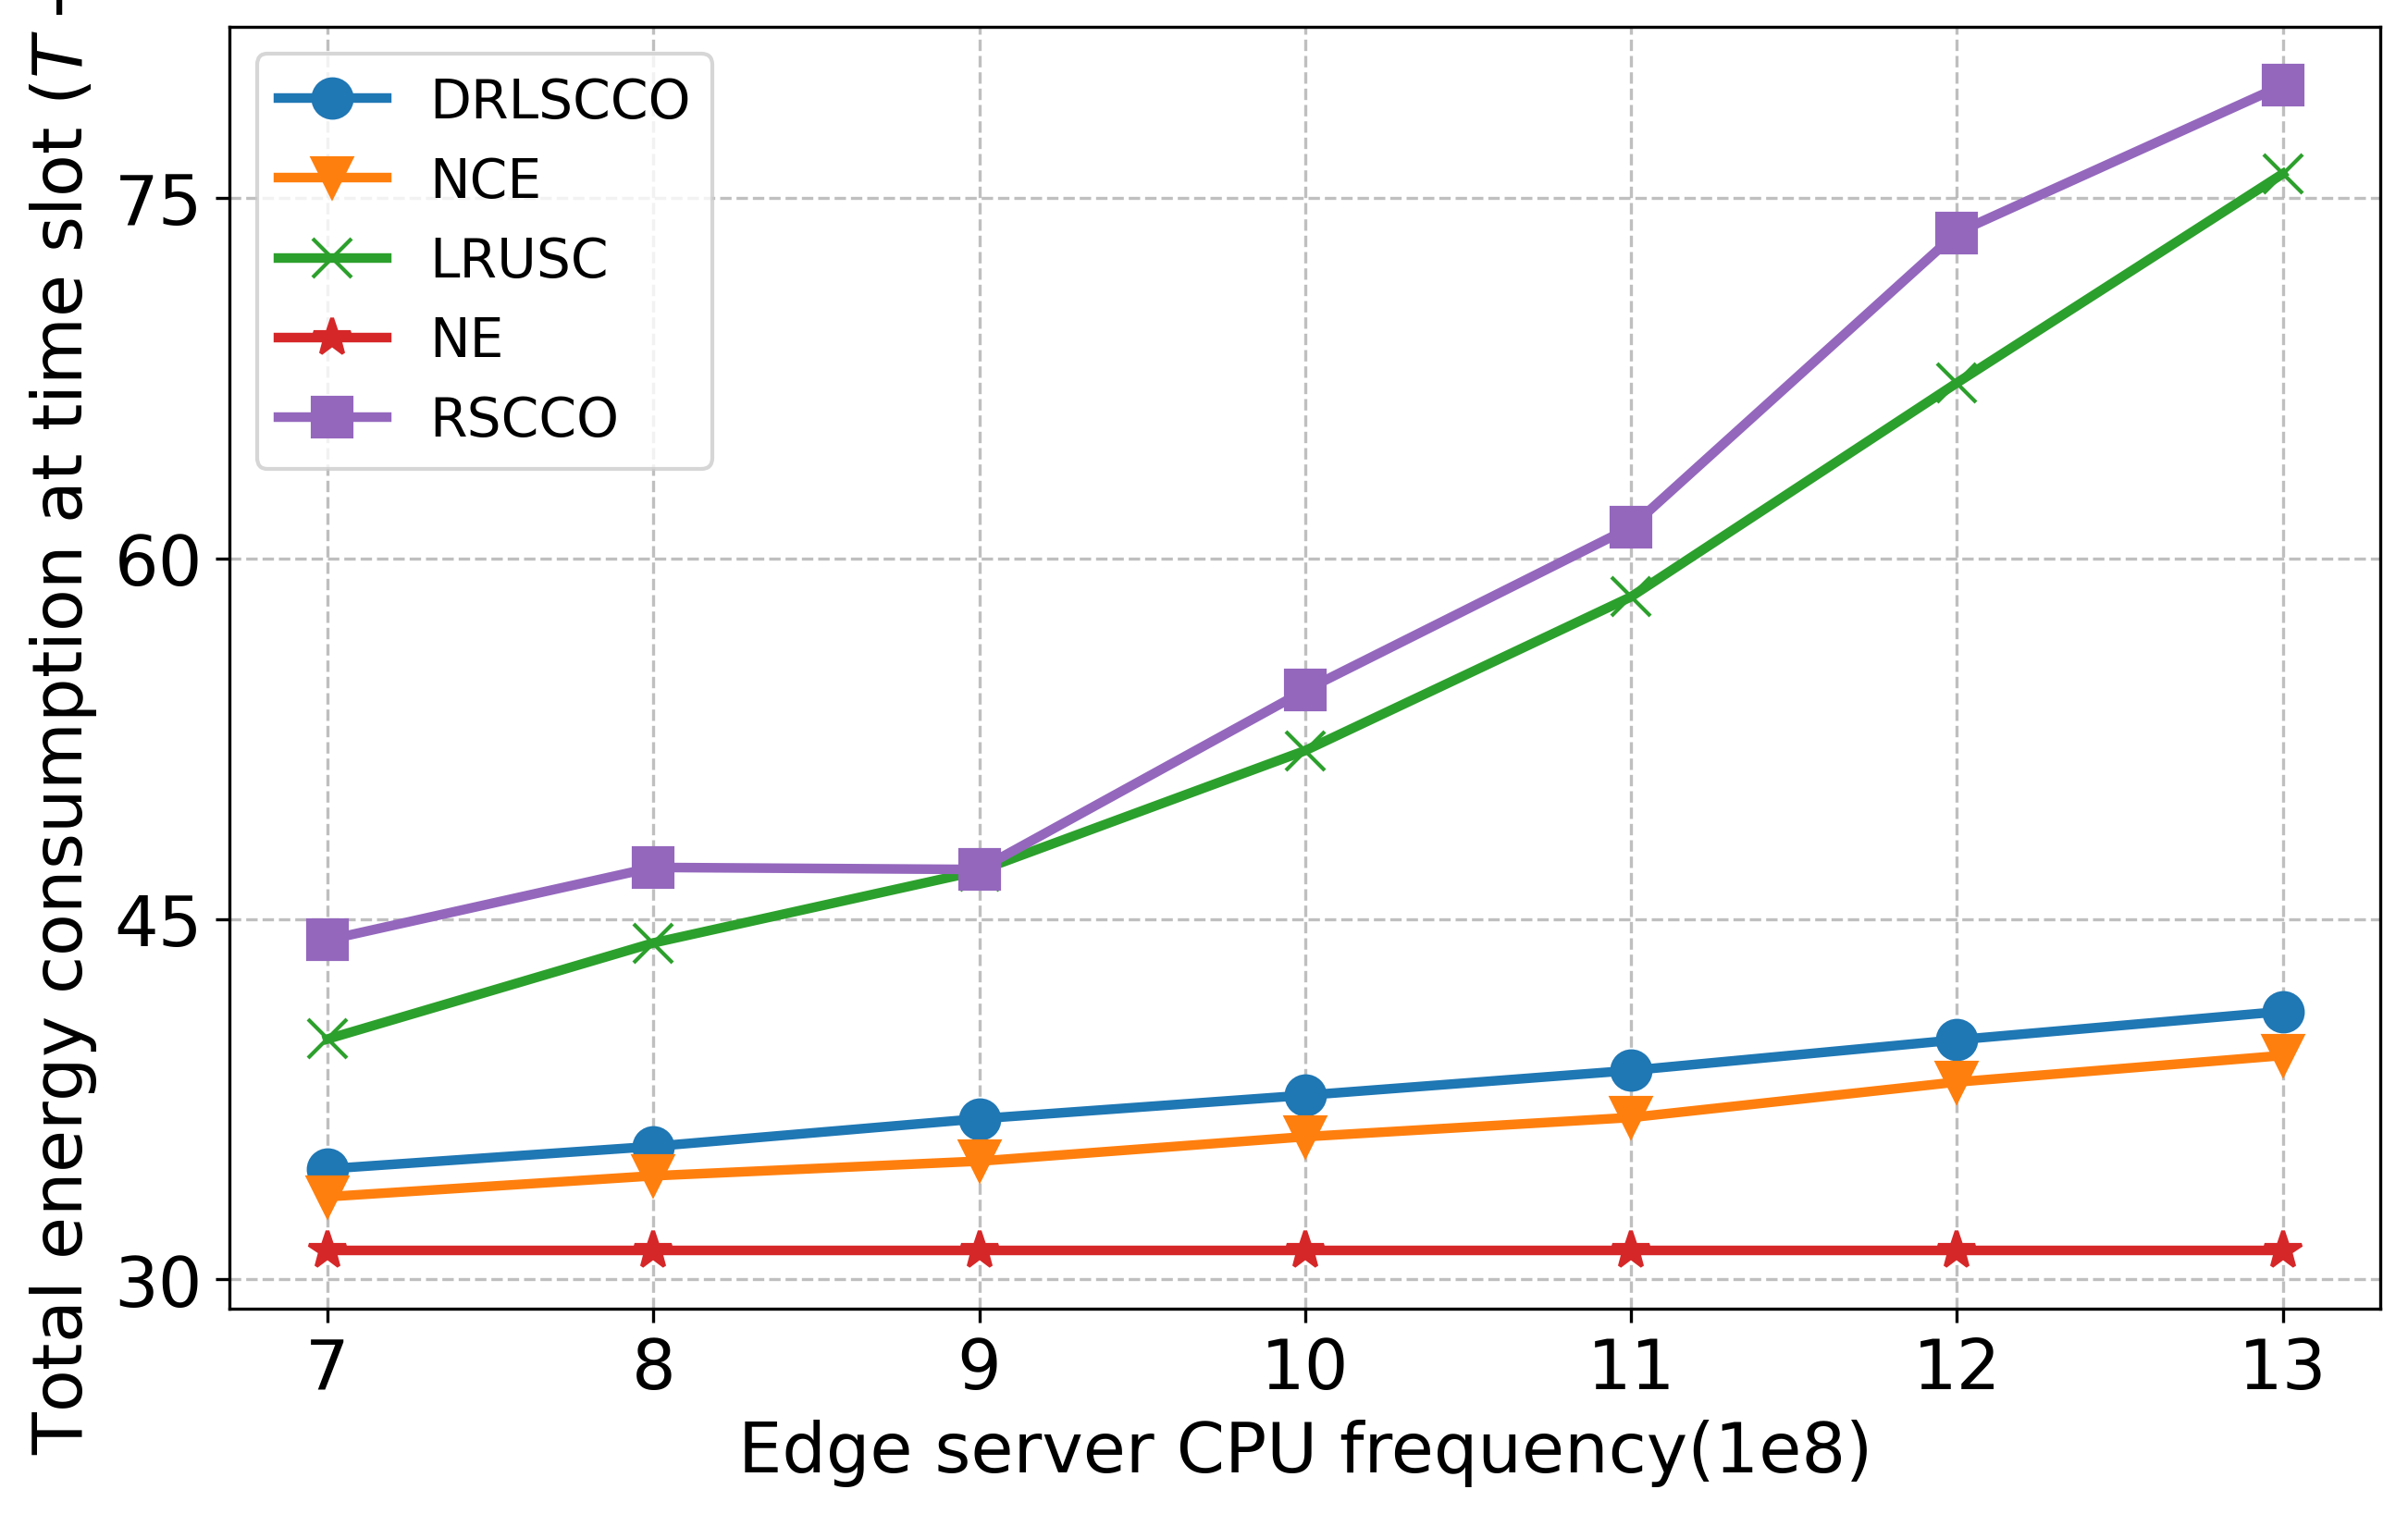
\includegraphics[width=3in]{f_energy.png}
	\caption{The influence of edge server's CPU frequency on energy}
	\label{fig: f v energy}
\end{figure}
The results in Fig. \ref{fig: f v delay} and Fig. \ref{fig: f v energy} align with theoretical expectations, demonstrating that higher CPU frequency enable lower task execution delay but also lead to increased  energy consumption. 
Since the NE scheme does not utilize edge servers, its delay and energy consumption remain constant regardless of CPU frequency changes.
The LRUSC scheme, which only implements the LRU strategy for service caching replacement without jointly optimizing service caching and task offloading, is less sensitive to variations in CPU frequency. 
Meanwhile, LRUSC generally exhibits lower delay and energy consumption compared to RSCCO, which lacks clear caching and offloading strategies and thus shows the most unstable performance with the highest delay.
Notably, when the CPU frequency is relatively low, the delays of LRUSC and RSCCO even exceed that of NE. This indicates that, under the same task size and vehicle density, the delay incurred by offloading subtask to cloud server may be lower than executing them on edge server with low computational capacity. 
However, as the CPU frequency increases to $6 \times 10^8$, the delays of LRUSC and RSCCO become lower than that of NE. Although the MNOs' energy consumption of LRUSC and RSCCO remains consistently higher than NE, this highlights that appropriate deployment of edge  computing capability by MNOs can significantly enhance user experience compared to relying solely on cloud computing.
In Fig. \ref{fig: f v delay}, it can be observed that for the proposed DRLSCCO scheme and the NCE scheme, the delays are relatively close when the CPU frequency is $4 \times 10^8$. As the CPU frequency increases, although the delay gap between DRLSCCO and NCE gradually widens, the growth rates of energy consumption for the two schemes remain nearly the same.
This phenomenon arises because when the edge computing capability is low, the subtask offloading among edge nodes in DRLSCCO causes additional transmission delays. Once the computational capacity becomes sufficient, this disadvantage diminishes. Moreover, since the MNO's energy consumption is closely related to computational delay, the energy consumption growth rate of DRLSCCO does not significantly exceed that of NCE.



\section{Conclusion}
This paper investigates a VEC system with limited edge caching resources, where each task depends on multiple types of services and tasks are decomposed into subtasks based on service requirements, resulting in a tightly coupled process between service caching and fine-grained task offloading.
We design the communication, caching, and offloading mechanisms, and model the execution delay and MNOs' energy consumption.
The joint service caching and subtask offloading problem is formulated as a MINLP problem, which is addressed using a DRL-based scheme, referred to as DRLSCCO.
Extensive simulation results demonstrate that DRLSCCO significantly reduces task execution delay while effectively balancing MNO energy consumption compared to several baseline methods.
For future work, potential research directions include addressing heterogeneous communication constraints, such as intermittent connectivity, and exploring decentralized or multi-agent learning frameworks to enhance system scalability and robustness.

\bibliographystyle{IEEEtran}
\bibliography{bib}
\end{document}
